% Created 2016-09-03 Sat 11:46
\documentclass[10pt, t]{beamer}
\usepackage[utf8]{inputenc}
\usepackage[T1]{fontenc}
\usepackage{fixltx2e}
\usepackage{graphicx}
\usepackage{longtable}
\usepackage{float}
\usepackage{wrapfig}
\usepackage{rotating}
\usepackage[normalem]{ulem}
\usepackage{amsmath}
\usepackage{textcomp}
\usepackage{marvosym}
\usepackage{wasysym}
\usepackage{amssymb}
\usepackage{hyperref}
\tolerance=1000
\usepackage{APC524b}
\addtobeamertemplate{frametitle}{}{\vspace{-3mm}}
\AtBeginSection[]{\stepcounter{subsection}\begin{frame}<beamer>\frametitle{Outline}\tableofcontents[currentsection]\end{frame}}
\let\sout=\code
\let\texttt=\graytt
\let\verb=\codeDelimTwiddles
\let\alert=\textbf
\lstset{language=python}
\usetheme{default}
\author{A. Svyatkovskiy, based on the original course by C. Rowley and R. Lupton}
\date{3 October 2016}
\title{Python}
\hypersetup{
  pdfkeywords={},
  pdfsubject={},
  pdfcreator={Emacs 24.5.1 (Org mode 8.2.7c)}}
\begin{document}

\maketitle
\begin{frame}{Outline}
\tableofcontents
\end{frame}


\section{Programming Languages}
\label{sec-1}
\begin{frame}{} %[label=sec-1-1]{Interpreted Languages}
%\begin{itemize}
%\item Fast development (no compile-link-run cycle)
%\item Interactive development
%\item High level (no need to worry about pointers)
%\end{itemize}
\begin{columns}
\column{1.1\linewidth}
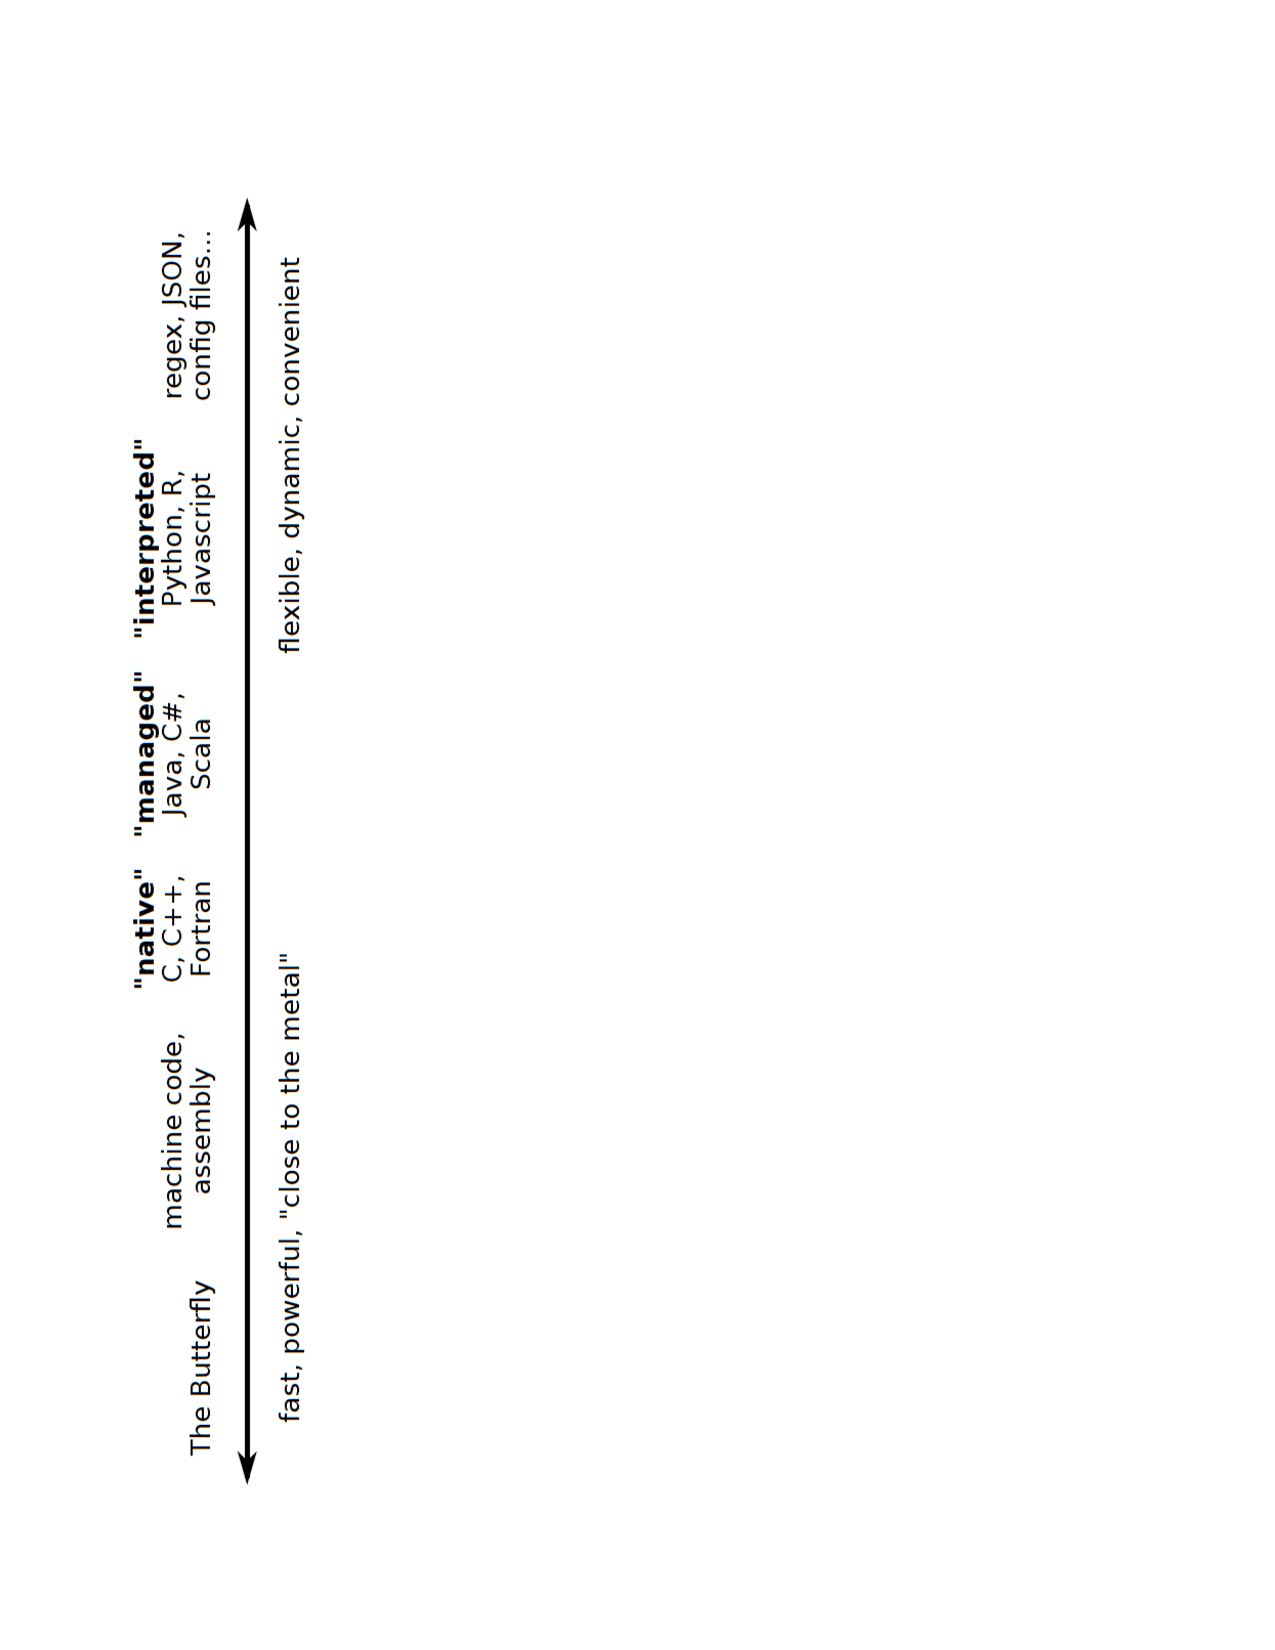
\includegraphics[angle=-90,width=\linewidth]{figures/languages1.pdf}
\end{columns}
\end{frame}

\begin{frame}{} %[label=sec-1-1]{Interpreted Languages}
%\begin{itemize}
%\item Fast development (no compile-link-run cycle)
%\item Interactive development
%\item High level (no need to worry about pointers)
%\end{itemize}
\begin{columns}
\column{1.1\linewidth}
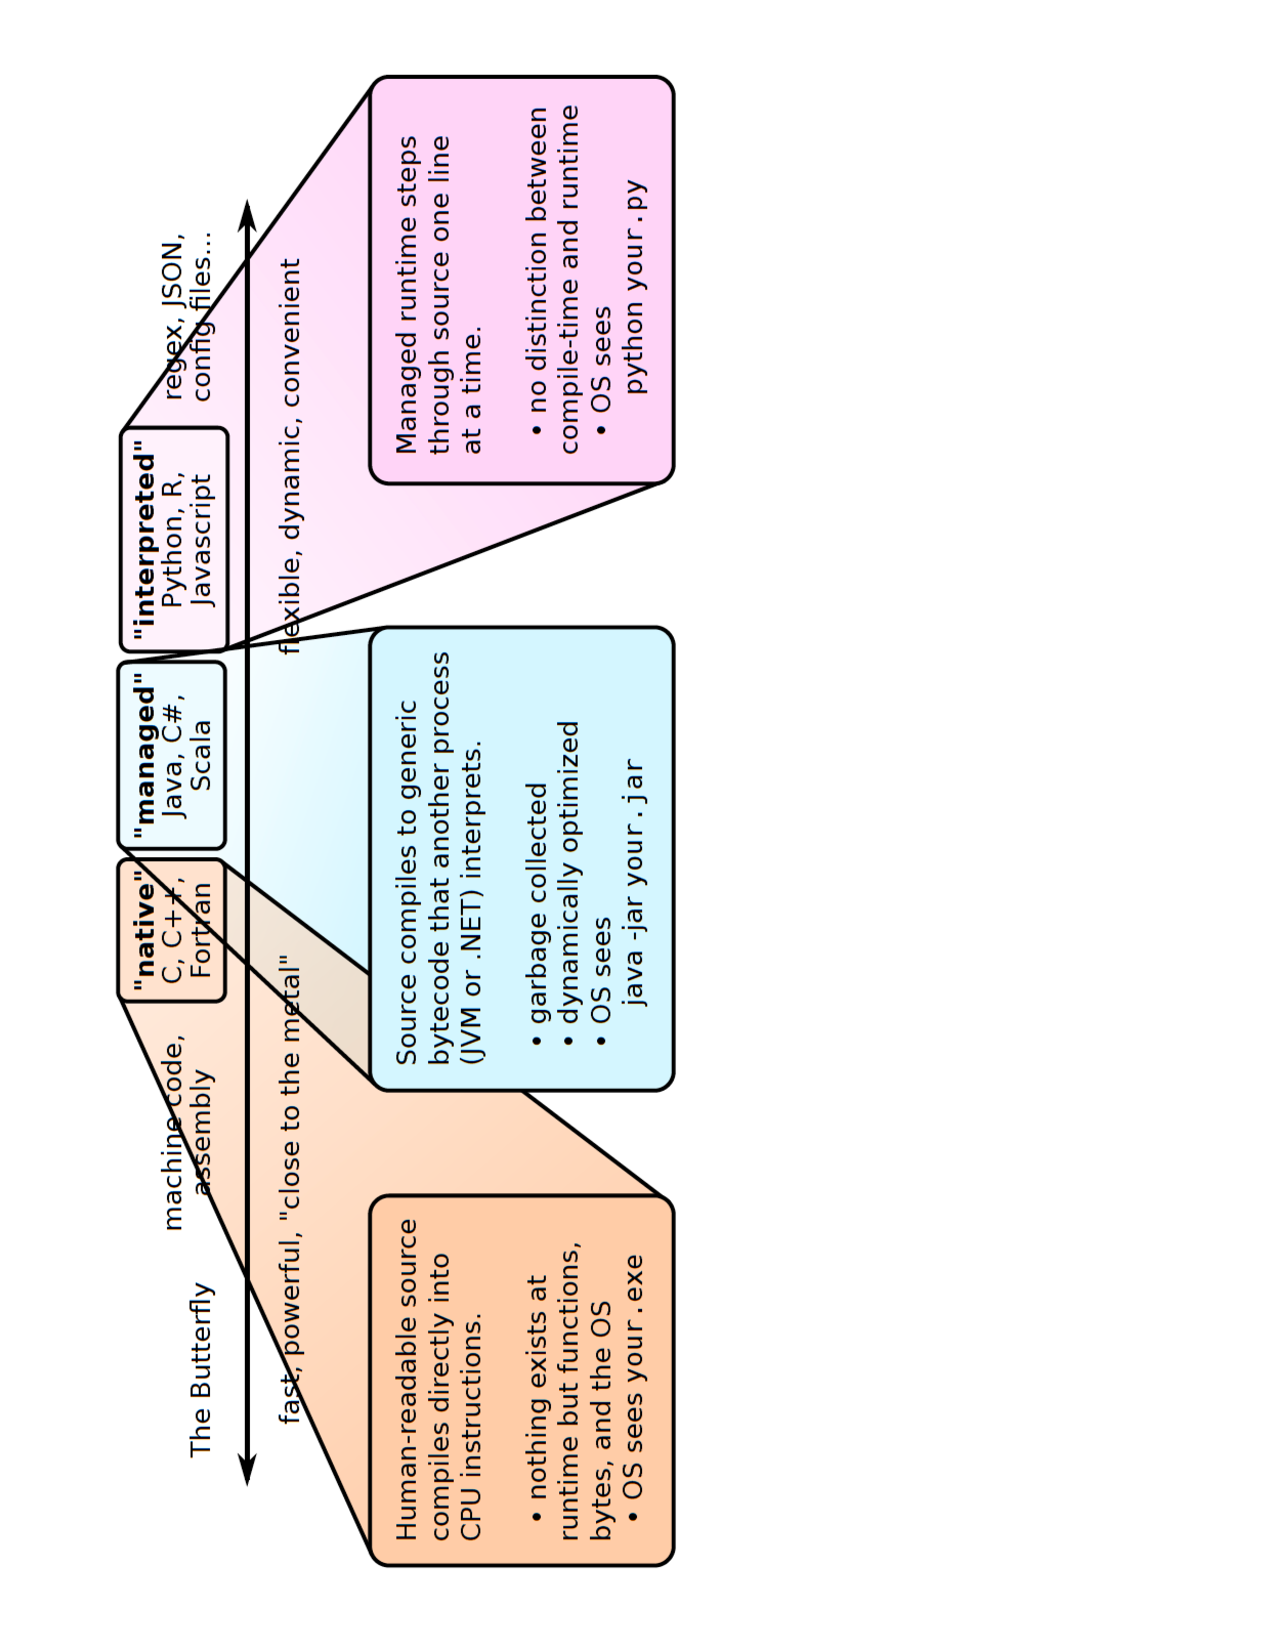
\includegraphics[angle=-90,width=\linewidth]{figures/languages2.pdf}
\end{columns}
\end{frame}

%\begin{frame}{} %[label=sec-1-1]{Interpreted Languages}
%\begin{itemize}
%\item Fast development (no compile-link-run cycle)
%\item Interactive development
%\item High level (no need to worry about pointers)
%\end{itemize}
%\begin{columns}
%\column{1.1\linewidth}
%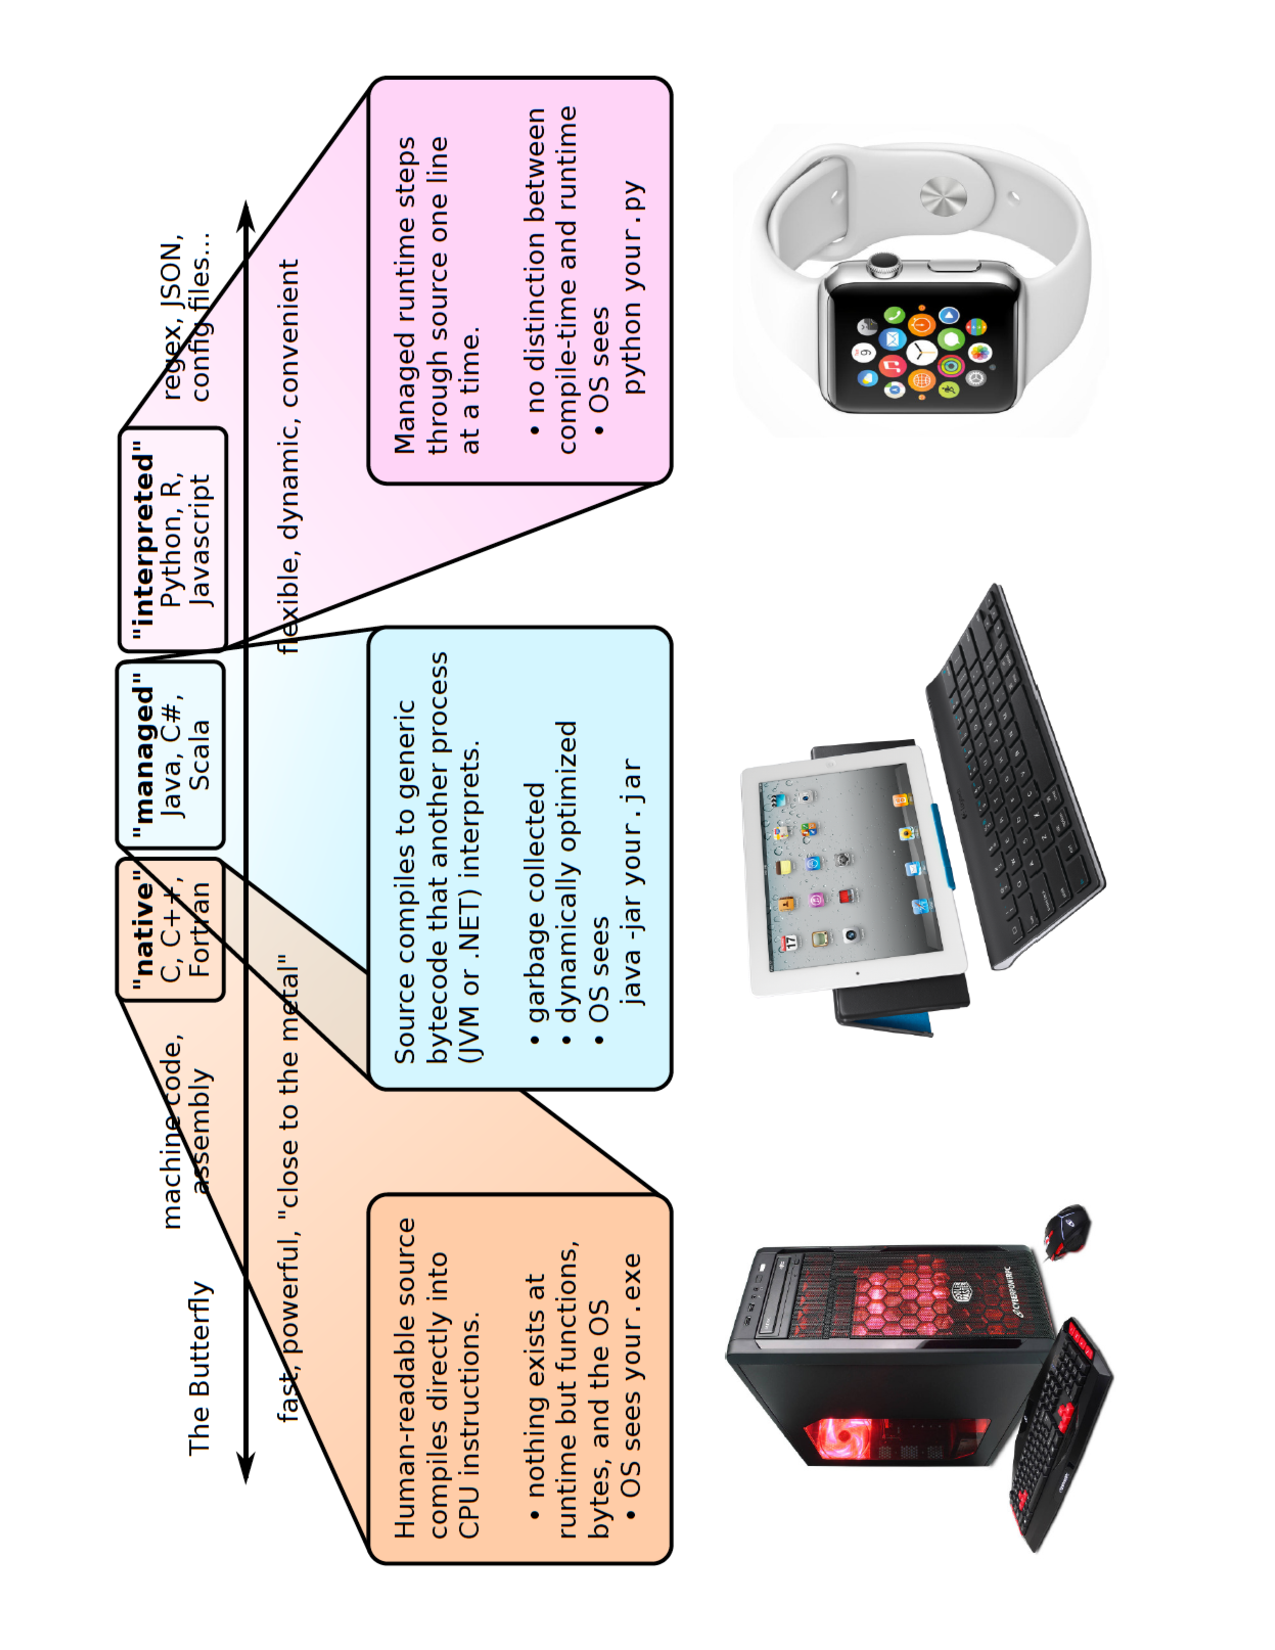
\includegraphics[angle=-90,width=\linewidth]{figures/languages3.pdf}
%\end{columns}
%\end{frame}

\begin{frame}{} %[label=sec-1-1]{Interpreted Languages}
%\begin{itemize}
%\item Fast development (no compile-link-run cycle)
%\item Interactive development
%\item High level (no need to worry about pointers)
%\end{itemize}
\begin{columns}
\column{1.1\linewidth}
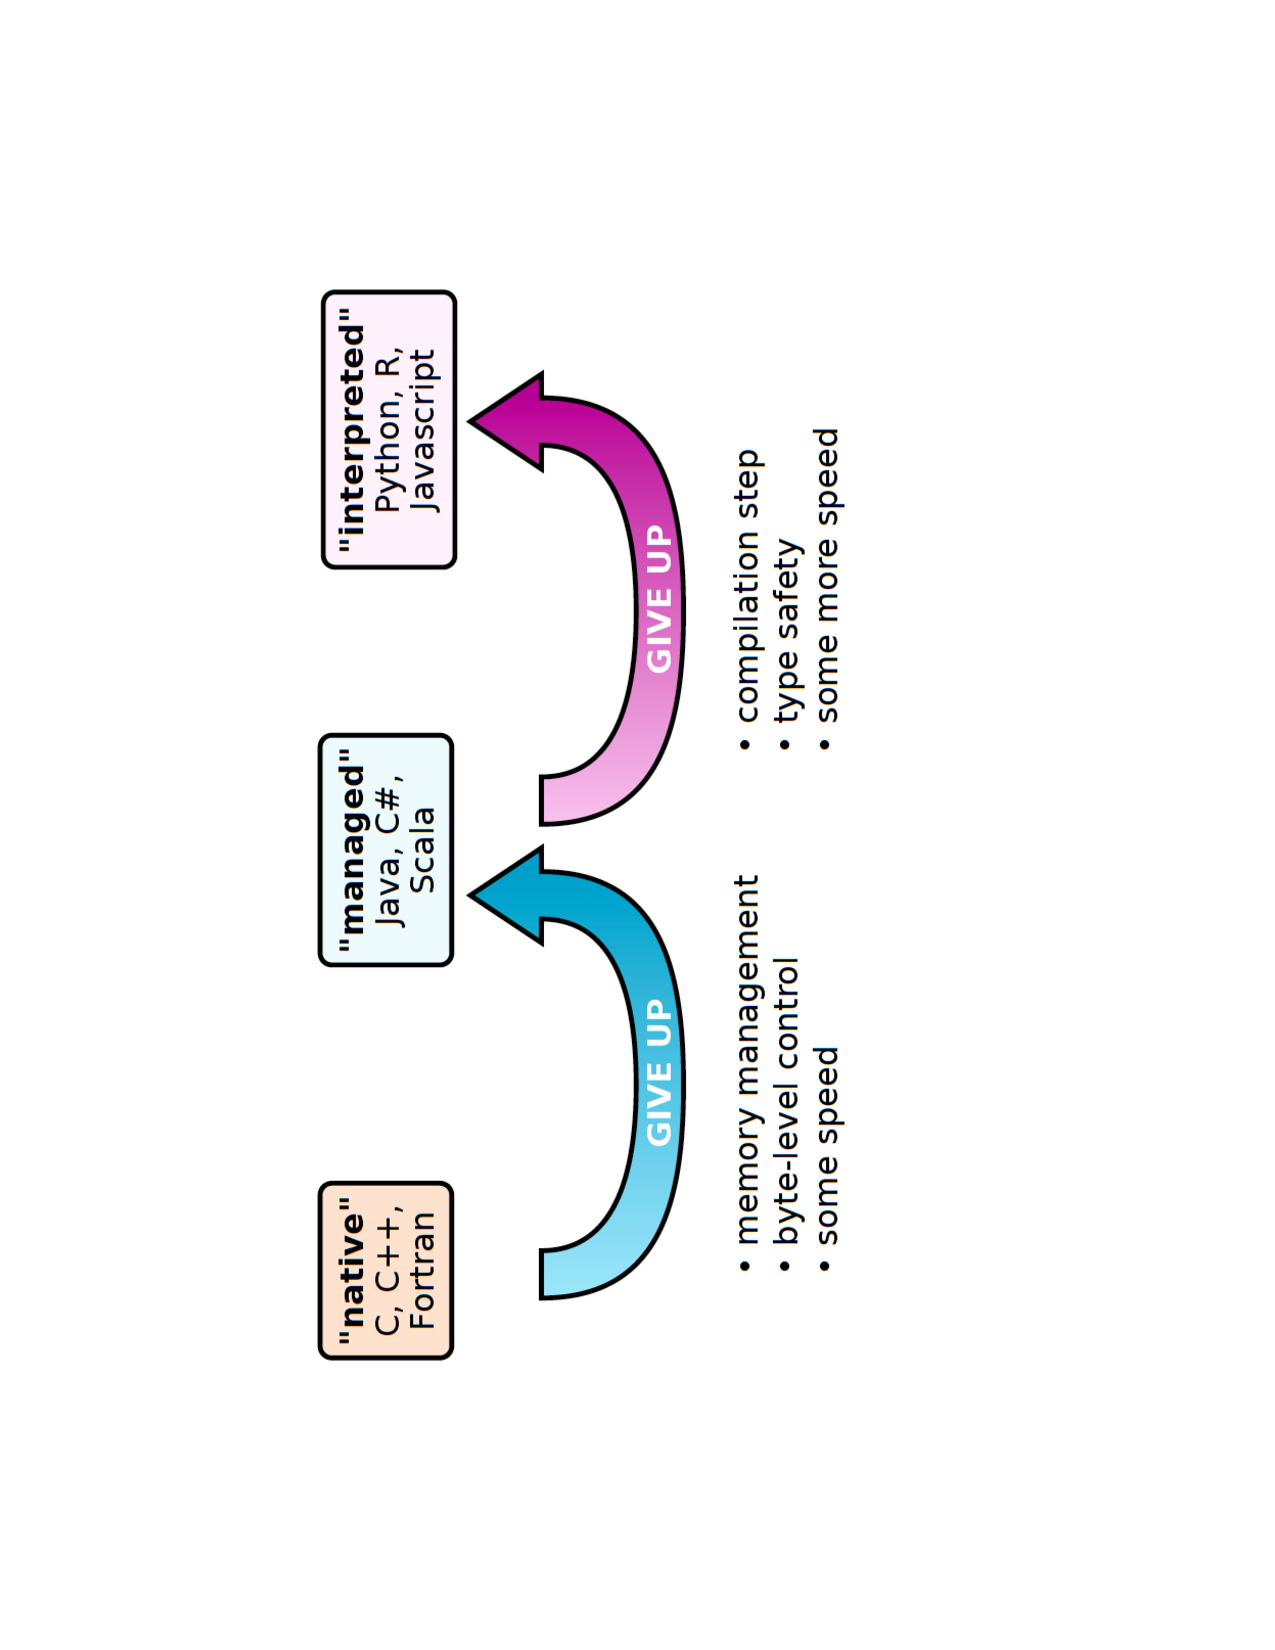
\includegraphics[angle=-90,width=\linewidth]{figures/languages4.pdf}
\end{columns}
\end{frame}

\begin{frame}{} %[label=sec-1-1]{Interpreted Languages}
%\begin{itemize}
%\item Fast development (no compile-link-run cycle)
%\item Interactive development
%\item High level (no need to worry about pointers)
%\end{itemize}
\begin{columns}
\column{1.1\linewidth}
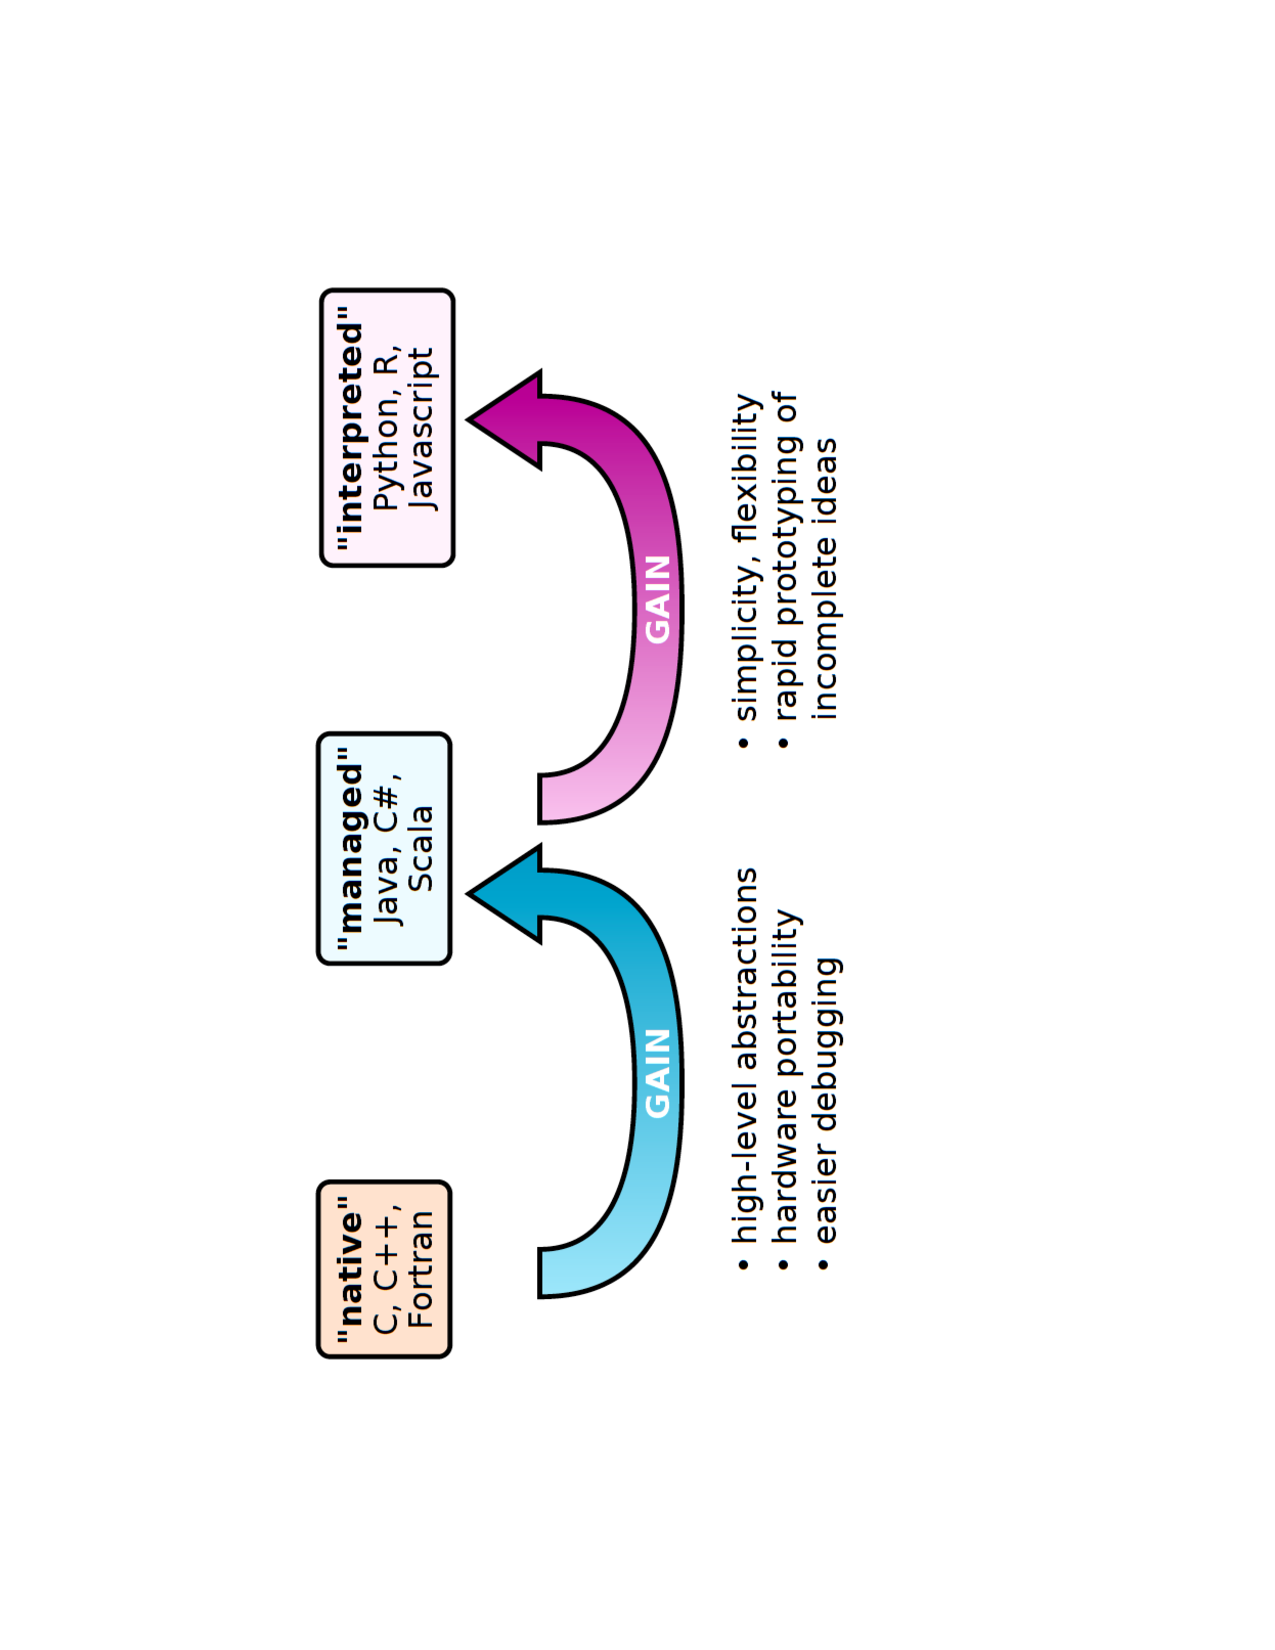
\includegraphics[angle=-90,width=\linewidth]{figures/languages5.pdf}
\end{columns}
\end{frame}


\begin{frame}[fragile,label=sec-1-2]{Python}
 \begin{itemize}
\item Powerful builtins
\item Object oriented
\item Rich libraries
\item Dynamic typing
\end{itemize}
\pause
\begin{block}{Official Tutorial and Manual}
\url{https://docs.python.org/2/tutorial/index.html}

\pause
\end{block}
\begin{block}{There are two slightly inconsistent versions of python in the wild, python \texttt{2.x} and python \texttt{3.x}}
\pause
Within the \texttt{2.x} series (currently \texttt{2.7.12}) features were added from time to time.  %If you're very concerned about
%portability you may want to avoid newer constructions (e.g. \verb~<x> if <logical> else <y>~, \verb~with~)
\pause
Eventually we'll all have to move to python 3 (currently at \texttt{3.5}).
\end{block}
\end{frame}

\section{Intro to Python}
\label{sec-2}
\begin{frame}[fragile,label=sec-2-2]{Hello World}
 Let us write "Hello world" in python:
\pause
\lstset{language=Python,label= ,caption= ,numbers=none}
\begin{lstlisting}
print "Hello world"
\end{lstlisting}
\pause
You can run python scripts from the shell:
\lstset{language=text,label= ,caption= ,numbers=none}
\begin{lstlisting}
$ cat hello.py
#!/usr/bin/env python
print "Hello world"
$ python hello.py
Hello world
\end{lstlisting}
(That \verb~\#!~ line is standard unix magic for, "use python to run this script";)

\pause
Or interactively:
\lstset{language=text,label= ,caption= ,numbers=none}
\begin{lstlisting}
$ python
>>> print "Hello world"
Hello world
\end{lstlisting}
\end{frame}
\begin{frame}[fragile,label=sec-2-3]{Interactive Usage}
 These days we are all spoilt by the unix shells.  \pause We expect:
\begin{itemize}
\item To be able to use $\uparrow \downarrow \leftarrow \rightarrow$ to save typing
\item To be able to use \verb~TAB~ to complete command and file names
\item That our history be saved between sessions
\end{itemize}
\pause
This is all available in python.  Two solutions:
\begin{itemize}
\item Put cunning and cryptic commands in your python startup file (\texttt{\$PYTHONSTARTUP})
\item Use \texttt{jupyter} interactive notebooks (\url{http://jupyter.org})
\end{itemize}
\pause
These days we definitely recommend \texttt{jupyter}.  You can install it from
\url{https://store.continuum.io/cshop/anaconda}
along with lots of other useful-to-essential packages, some of which we'll discuss today.

\pause
On \texttt{nobel.princeton.edu} you can use \texttt{python} \texttt{2.7} and \texttt{jupyter 4.1.1} by saying \texttt{module load anaconda}
(maybe in your \alert{.bashrc} file).  If you find other Princeton machines where this doesn't work please
let CSES know.
\end{frame}

\begin{frame}[fragile,label=sec-2-4]{Primitive types}
 \begin{itemize}
\item \verb~None~
\item \verb~bool~ (\verb~True~, \verb~False~)
\item \verb~int~
\item \verb~long~ (arbitrary precision)
\item \verb~float~
\end{itemize}
\end{frame}
\begin{frame}[fragile,label=sec-2-5]{Lists and Tuples}
 Python supports two separate-but-almost-equal list types:
\begin{itemize}
\item \verb~list~
\end{itemize}
\lstset{language=Python,label= ,caption= ,numbers=none}
\begin{lstlisting}
>>> li = [100, 101, 102, 103]
>>> li[0]
100
>>> x = li[1:3]
>>> x
[101, 102]                              # not [100, 101, 102]
\end{lstlisting}
\pause
\lstset{language=Python,label= ,caption= ,numbers=none}
\begin{lstlisting}
>>> li[-1] = 666
>>> li
[100, 101, 102, 666]
\end{lstlisting}
Useful list methods: \verb~append~, \verb~insert~, \verb~pop~, \verb~reverse~, \verb~sort~, \verb~index~
\pause
\begin{itemize}
\item \verb~tuple~: a list that is "frozen" and cannot be changed (immutable)
\end{itemize}
\lstset{language=Python,label= ,caption= ,numbers=none}
\begin{lstlisting}
>>> tp = (100, 101, 102, 103)
>>> tp[0]
100
>>> x = tp[1:3]
>>> x
(101, 102)
\end{lstlisting}
\pause
\lstset{language=Python,label= ,caption= ,numbers=none}
\begin{lstlisting}
>>> tp[-1] = 666
Traceback (most recent call last):
  File "<stdin>", line 1, in <module>
TypeError: 'tuple' object does not support item assignment
\end{lstlisting}

%FIXME
%\pause
%\begin{itemize}
%\item \verb~set~: a list with each element appearing only once.
%\end{itemize}
\end{frame}
\begin{frame}[fragile,label=sec-2-6]{Strings}
 Python strings can be delimited with \code{"}, \code{'}, \code{"""}, or  \code{'''}
\lstset{language=Python,label= ,caption= ,numbers=none}
\begin{lstlisting}
>>> s = "Hello world"
>>> s2 = 'Goodbye, sweet life'
>>> s3 = """I really like
to split greetings over multiple lines"""
\end{lstlisting}
(there's no difference between \code{"} and \code{'}, unlike the unix shells).
\pause
I recommend \alert{not} randomly switching between  \code{"} and \code{'} strings (as it makes it hard to
find them in your editor).  I personally follow the C convention: \code{"Hello world"} but \code{'H'}.
\pause 
Sometimes.

\pause
Strings have several useful methods:
\lstset{language=Python,label= ,caption= ,numbers=none}
\begin{lstlisting}
>>> print s.upper()
HELLO WORLD
\end{lstlisting}
\pause
\lstset{language=Python,label= ,caption= ,numbers=none}
\begin{lstlisting}
>>> s.find('w')
6
\end{lstlisting}
\pause
\lstset{language=Python,label= ,caption= ,numbers=none}
\begin{lstlisting}
>>> print s[s.find('w'):]
world
\end{lstlisting}
\pause
\lstset{language=Python,label= ,caption= ,numbers=none}
\begin{lstlisting}
>>> s.split()
['Hello', 'world']
\end{lstlisting}
\pause
%FIXME
%You can't interpolate variable (\code{"\$a \$b \$c"}), but you can say
%\lstset{language=Python,label= ,caption= ,numbers=none}
%\begin{lstlisting}
%>>> a, b, c = "A", "B", "C"
%>>> print "%s %s %s" % (a, b, c)
%A B C
%\end{lstlisting}
\end{frame}

\begin{frame}[fragile,label=sec-2-7]{Dictionaries}
 \lstset{language=Python,label= ,caption= ,numbers=none}
\begin{lstlisting}
>>> di = {"alexeys":"Alexey", "cwrowley":"Clancy", "jmstone":"Jim"}
>>> di.update({"rhl" : "Robert"}}
>>> di.update({'rhl':'Robert'})
>>> di
{'cwrowley': 'Clancy', 'jmstone': 'Jim', 'alexeys': 'Alexey', 'rhl': 'Robert'}
\end{lstlisting}
\pause
\lstset{language=Python,label= ,caption= ,numbers=none}
\begin{lstlisting}
>>> print di['rhl']
Robert
>>> print di.keys(), di.values()
['cwrowley', 'rhl', 'jmstone'] ['Clancy', 'Robert', 'Jim']
\end{lstlisting}
\pause
\lstset{language=Python,label= ,caption= ,numbers=none}
\begin{lstlisting}
>>> di = dict(president = "Obama")
\end{lstlisting}
\pause
\lstset{language=Python,label= ,caption= ,numbers=none}
\begin{lstlisting}
>>> di["president"] = "Eisgruber"
>>> di["provost"] = "Lee"
\end{lstlisting}
\pause
\emph{N.b.} python supports \emph{garbage collection}; when we said \code{di = dict(president = "Obama")} the memory for
our email dictionary was returned to the system.

\pause
You can use dictionaries in conjunction with \code{\%} formatting:
\lstset{language=Python,label= ,caption= ,numbers=none}
\begin{lstlisting}
>>> foods = dict(a="Apple", b="Banana", c="Carrot")
>>> print "%(a)s %(b)s %(c)s" % foods
Apple Banana Carrot
\end{lstlisting}

\pause
This style \code{\%} formatting is actually deprecated in python \verb~>= 2.6~; 
you're supposed to say things like
\lstset{language=Python,label= ,caption= ,numbers=none}
\begin{lstlisting}
"{0} {1} {c}".format("Apple", "Banana", c="Carrot")
\end{lstlisting}
but this seems pretty clunky to me.
\pause
It seems unlikely that \code{\%} formatting will ever go away.
\end{frame}

\begin{frame}[fragile,label=sec-2-8]{Mix and Match}
 There is no restriction that the elements of any of these data types be simple.
\pause
\lstset{language=Python,label= ,caption= ,numbers=none}
\begin{lstlisting}
>>> addressBook = {}
>>> addressBook["Alexey"] = ["alexeys", "Svyatkovskiy"]
>>> addressBook["Robert"] = ["rhl", "Lupton"]
>>> print addressBook["Alexey"][0]
alexeys
\end{lstlisting}
\pause
\lstset{language=Python,label= ,caption= ,numbers=none}
\begin{lstlisting}
>>> addressBook = {}
>>> addressBook["Alexey"] = dict(email = "alexeys", surname = "Svyatkovskiy")
>>> addressBook["Robert"] = {}
>>> addressBook["Robert"]["email"] = "rhl"
>>> addressBook["Robert"]["surname"] = "Lupton"
>>> print addressBook["Robert"]["email"]
rhl
\end{lstlisting}

\pause
You can't use a \verb~list~ as a key in a \verb~dict~ (as you might modify the list later), but you \emph{can} use a \verb~tuple~
as it's immutable.
\end{frame}

\begin{frame}[fragile,label=sec-2-9]{Loading source files}
 If you have a file \alert{foo.py}, you can make it visible from python with \verb~import foo~.  If you modify
\alert{foo.py} and repeat the import, nothing happens.
\pause To see your changes, you have to say \verb~reload(foo)~

\pause
Python searches for \alert{foo.py} by searching the directories in \texttt{\$PYTHONPATH} (a \verb~:~ separated list)
in order.
\pause
When you first \verb~import~ a file it's compiled to a \emph{.pyc} file (\alert{foo.pyc}).  You'll probably want to tell
your source code manager (e.g. \verb~git~) to ignore \emph{.pyc} files, \emph{e.g.} by adding \texttt{*.pyc} to 
your \alert{.gitignore} file.

\pause
"Orphan" \textit{.pyc} files can be very confusing.
\pause
If you move \alert{foo.py} to a directory later in \texttt{\$PYTHONPATH}, but leave \alert{foo.pyc} behind, python will happily import 
the \emph{.pyc} file for you;  this may not be what you intended.
\pause
Examining \verb~foo.\_\_file\_\_~ can help diagnose the problem.
\end{frame}

\begin{frame}[fragile,label=sec-2-10]{Control structures}
 Python has the standard control structures: \verb~if-elif-else~, \verb~for~, \verb~while~ and logicals \verb~and~, \verb~or~, 
\verb~not~ \verb~==~, \verb~<~, \ldots{}
\lstset{language=Python,label= ,caption= ,numbers=none}
\begin{lstlisting}
  if x == 1:
      print "One"
  elif x == 2 or x == 3:
      print "Two or Three"
  else:
      print "Something else"
\end{lstlisting}
The block structure is \emph{defined} by whitespace.
\pause This seems weird, but you soon get used to it.
%\pause I believe that it was a very bad design decision, but it's not going to change.

\pause
Because there isn't any information about a program's block structure except the white space, you 
have to be very careful.  

\pause 
Another issue is mixing tabs and spaces;  it's probably better to instruct your editor to insert spaces even 
when you hit the tab key to avoid the problem.
\end{frame}
%\begin{frame}[fragile,label=sec-2-11]{Changing program logic}
% In C I can write
%\lstset{language=C,label= ,caption= ,numbers=none}
%\begin{lstlisting}
%  if (x == 1) {
%     printf("One\n");
%  } else {
%     printf("Not one\n");
%  }
%\end{lstlisting}
%\pause
%If I need to change the indentation level I can modify this to
%\lstset{language=C,label= ,caption= ,numbers=none}
%\begin{lstlisting}
%  if (y == 10) {
%  if (x == 1) {
%     printf("One\n");
%  } else {
%     printf("Not one\n");
%  }
%  }
%\end{lstlisting}
%and get my editor to reindent to make it look pretty.

%\pause
%In python, things aren't so nice.
%\pause
%\lstset{language=Python,label= ,caption= ,numbers=none}
%\begin{lstlisting}
%  if y == 10:
%  if x == 1:
%      print("One")
%  else:
%      print("Not one")
%\end{lstlisting}
%I cannot tell whether the \verb~else~ belongs to the \verb~x~ or \verb~y~ test.
%\pause
%My only hope is to rigidly reindent the block (use \code{^C>} in emacs)
%\end{frame}

\begin{frame}[fragile,label=sec-2-12]{\verb~for~ and \verb~while~ loops}
 \lstset{language=Python,label= ,caption= ,numbers=none}
\begin{lstlisting}
for r in ("Arrow", "Birdland", "Matinee"):
   print r
\end{lstlisting}
\pause
\lstset{language=Python,label= ,caption= ,numbers=none}
\begin{lstlisting}
n = 10
for i in range(n):
   for j in range(i, n):
      print i, j
\end{lstlisting}
(note that \verb~range(n)~ counts from \verb~0~ to \verb~n-1~, not up to \verb~n~).
\pause
\lstset{language=Python,label= ,caption= ,numbers=none}
\begin{lstlisting}
i = 0
while True:
   i += 10
   if i == 100:
      break
   print i
\end{lstlisting}
\pause \verb~continue~ is also available.
\pause But \verb~goto~ isn't.

\pause
\alert{Warning}: Looping over strings can do the wrong thing
\lstset{language=Python,label= ,caption= ,numbers=none}
\begin{lstlisting}
>>> for c in ("abc",): print c
abc
\end{lstlisting}
\pause
\lstset{language=Python,label= ,caption= ,numbers=none}
\begin{lstlisting}
>>> for c in ("abc"): print c
a
b
c
\end{lstlisting}
\pause
That comma is essential.  
It isn't really the loop's fault, it's just that a string is treated as a list of characters.
\end{frame}

\begin{frame}[fragile,label=sec-2-13]{Functions}
 \lstset{language=Python,label= ,caption= ,numbers=none}
\begin{lstlisting}
def simple_squares(n):
    squares = []
    for number in range(n):
        squares.append(number*number)
        # Now, squares should have [1,4,9,16,25]
    print "List of squares: ", squares
\end{lstlisting}
\pause
Simple variables (\verb~int~, \verb~float~) are passed by \emph{value}; everything else is passed by \emph{reference}.

\pause
This mans that if you modify a list or dictionary passed to a function it'll be modified in the calling routine too; 
you may need to make a copy:
\lstset{language=C,label= ,caption= ,numbers=none}
\begin{lstlisting}
li = li[:]
di = di.copy()
\end{lstlisting}
It'd be nice if \verb~list~ also supported \verb~copy~, the closest is \verb~list(xxx)~.
You can always use \verb~import copy; copy.copy(xxx)~ (but it's slower).
\pause
This is a \emph{shallow copy}, but \verb~copy.deepcopy~ is also available.
\end{frame}

\begin{frame}[fragile,label=sec-2-13-1]{Lambda Functions}
 \lstset{language=Python,label= ,caption= ,numbers=none}
Python supports anonymous functions using a construct called "lambda".
Sometimes you need to pass a function as an argument, or you want to do a short but complex operation multiple times. Following lambda is completely identical to the function defined on the previous slide:
\begin{lstlisting}
def simple_squares_lambda(n):
    squares = map(lambda x: x*x, range(n))
    print "List of squares calculated in a Pythonic way with lambda: ", squares
\end{lstlisting}
\pause
Lambda functions are typically used in functional programming languages like Scala and in frameworks like Spark.
\end{frame}

\begin{frame}[fragile,label=sec-2-16]{Functional programming}
\emph{map}, \emph{filter}, \emph{reduce} functions facilitate a functional approach to programming
in Python: 
\lstset{language=Python,label= ,caption= ,numbers=none}
\begin{lstlisting}
def functional_python(n):
    squares = map(lambda x: x*x, filter(lambda x: x < 4, range(n)))
    return squares
\end{lstlisting}
\end{frame}
\pause
Here is a \emph{reduce} example that calculates sum of integers in a list:
\lstset{language=Python,label= ,caption= ,numbers=none}
\begin{lstlisting}
>>>reduce(lambda x,y: x+y, [47,11,42,13])
113
\end{lstlisting}
\end{frame}

\begin{frame}[fragile,label=sec-2-14]{Hello World}
 A better \alert{hello.py} script is
\lstset{language=text,label= ,caption= ,numbers=none}
\begin{lstlisting}
$ cat hello.py
#!/usr/bin/env python
def greet(who="world")
   print "Hello %s" % (who)

if __name__ == "__main__":
   greet()
\end{lstlisting}
\pause
The advantage is that I can say either
\lstset{language=text,label= ,caption= ,numbers=none}
\begin{lstlisting}
$ python hello.py
Hello world
\end{lstlisting}
or
\lstset{language=Python,label= ,caption= ,numbers=none}
\begin{lstlisting}
>>> import hello
>>> hello.greet("class")
Hello class
\end{lstlisting}
(\verb~\_\_name\_\_~ is
\code{"__main__"}
when run from the shell, and 
\code{"hello"}
when imported).
\end{frame}

\begin{frame}[fragile,label=sec-2-15]{Default arguments}
 You can also specify default values for arguments (as well as variable numbers of arguments):
\lstset{language=Python,label= ,caption= ,numbers=none}
\begin{lstlisting}
  def my_range(n, end=None, dn=1):
     """Return a list of numbers 
  Details ...
  """
     if end is None:
        i, end = 0, n
     else:
        i = n
    
     out = []
     while i < end:
        out.append(i)
        i += dn
    
     return out
\end{lstlisting}
\pause
\lstset{language=Python,label= ,caption= ,numbers=none}
\begin{lstlisting}
>>> my_range(3)
(0, 1, 2)
>>> my_range(2, 4)
(2, 3)
>>> my_range(2, 10, 2)
(2, 4, 6, 8)
>>> my_range(10, dn=2)
(0, 2, 4, 6, 8)
\end{lstlisting}
\end{frame}
\begin{frame}[fragile,label=sec-2-16]{List comprehensions}
 \lstset{language=Python,label= ,caption= ,numbers=none}
\begin{lstlisting}
>>> print [10 + x for x in range(5)]
[10, 11, 12, 13, 14]
\end{lstlisting}

\pause
\lstset{language=Python,label= ,caption= ,numbers=none}
\begin{lstlisting}
print [10 + x for x in range(5) if x%2 == 0]
[10, 12, 14]
\end{lstlisting}
\pause

This is surprisingly useful
\pause

If you write instead
\lstset{language=Python,label= ,caption= ,numbers=none}
\begin{lstlisting}
>>> r = (10 + x for x in range(5))
\end{lstlisting}
you get a \emph{generator} instead:
\lstset{language=Python,label= ,caption= ,numbers=none}
\begin{lstlisting}
>>> print r
<generator object <genexpr> at 0x1005cde10>
\end{lstlisting}
\pause
\lstset{language=Python,label= ,caption= ,numbers=none}
\begin{lstlisting}
>>> print [x for x in r]
[10, 11, 12, 13, 14]
>>> print list(r)
[10, 11, 12, 13, 14]
\end{lstlisting}
See the next slide for an explanation.
\end{frame}

%FIXME
\begin{frame}[fragile,label=sec-2-16]{Dictionary comprehensions}
 \lstset{language=Python,label= ,caption= ,numbers=none}
A dictionary comprehension takes the form \emph{{key: value for (key, value) in iterable}}. 
This syntax was introduced in Python 3 and backported to Python 2.7. 
Main use case is given two lists to create a dictionary where the item at each position in the first list becomes a key and the item at the corresponding position in the second list becomes the value:
\begin{lstlisting}
>>> seasons = ['Fall','Winter','Spring','Summer']
>>> {k[:2]: v for (k, v) in zip(seasons, range(len(seasons)))}
{'Fa': 0, 'Sp': 2, 'Su': 3, 'Wi': 1}
\end{lstlisting}
\end{frame}

\begin{frame}[fragile,label=sec-2-17]{Generators and iterators}
 Consider
\lstset{language=Python,label= ,caption= ,numbers=none}
\begin{lstlisting}
def fibonacci(n):
    prev = 0
    cur = 1
    for j in range(n):
        @\color{red}yield@ cur
        (cur, prev) = (cur + prev, cur)
\end{lstlisting}
\pause
\lstset{language=Python,label= ,caption= ,numbers=none}
\begin{lstlisting}
>>> [x for x in fibonacci(10)]
[1, 1, 2, 3, 5, 8, 13, 21, 34, 55]
\end{lstlisting}

\pause

\verb~fibonacci~ returns a \emph{generator} which has a method \verb~next~. The first call to \verb~next~ calls \verb~fibonacci~ and returns
the value of the \verb~yield~ statement.  When you call \verb~next~ again it miraculously resumes just after the \verb~yield~
and continues until it reaches \verb~yield~ again; when it \verb~returns~ (either explicitly or implicitly) a
\verb~StopIteration~ exception is raised:

\pause
\lstset{language=Python,label= ,caption= ,numbers=none}
\begin{lstlisting}
>>> f = fibonacci(1)
>>> f.next()
1
>>> f.next()
Traceback (most recent call last):
  File "<stdin>", line 1, in <module>
StopIteration
\end{lstlisting}
\end{frame}

\begin{frame}[fragile,label=sec-2-18]{Exceptions}
 Don't do this at home:
\lstset{language=Python,label= ,caption= ,numbers=none}
\begin{lstlisting}
>>> my_range(0, 10, -2)
\end{lstlisting}
\pause
the program will appear to hang until you hit \verb~\^C~ (or run out of memory --- I 
should have used \verb~yield~)
\pause 

\lstset{language=Python,label= ,caption= ,numbers=none}
\begin{lstlisting}
>>> ^C^C
>>> import pdb;  pdb.pm()
0
0
> <stdin>(13)my_range()
(Pdb) p i
-5184308
(Pdb)
\end{lstlisting}
We're counting down to $-\infty$

\pause
\lstset{language=Python,label= ,caption= ,numbers=none}
\begin{lstlisting}
  def my_range(n, end=None, dn=1):
     ...
     if end > n and dn <= 0:
        raise RuntimeError("Increment is negative: %g" % (dn))
\end{lstlisting}
\end{frame}
\begin{frame}[fragile,label=sec-2-19]{Catching exceptions}
 An exception need not be fatal:
\lstset{language=Python,label= ,caption= ,numbers=none}
\begin{lstlisting}
try:
   my_range(0, 10, -2)
except RuntimeError, e:
   print "Caught exception:", e
\end{lstlisting}
\pause
There are also more complicated and powerful forms of this \verb~try~ \verb~except~ pattern.
\end{frame}
\begin{frame}[fragile,label=sec-2-20]{Classes}
 Python is an Object Oriented language.
In \alert{people.py} I wrote:
\lstset{language=Python,label= ,caption= ,numbers=none}
\begin{lstlisting}
  class Person(object):
      """Describe a person"""
  
      def __init__(self, email=None, surname=None):
          self.email = email
          self.surname = surname
\end{lstlisting}
\pause
Note that \verb~self~ plays the part of \CPP's \verb~this~, but you have to explicitly write it out.  All member
functions expect \verb~self~ as their first argument.
\pause Let's use our new \verb~class~
\lstset{language=Python,label= ,caption= ,numbers=none}
\begin{lstlisting}
>>> import people
>>> addressBook = {}
>>> addressBook["Clancy"] = people.Person("cwrowley", "Rowley")
>>> addressBook["Robert"] = people.Person(surname="Lupton")
>>> print addressBook["Clancy"].email
cwrowley
\end{lstlisting}
\end{frame}
\begin{frame}[fragile,label=sec-2-21]{Special Methods}
 Let's take a look at Clancy:
\lstset{language=Python,label= ,caption= ,numbers=none}
\begin{lstlisting}
>>> print addressBook["Clancy"]
<people.Person object at 0x10056cd90>
\end{lstlisting}
\pause
That's annoying.  The solution is to add a method \verb~\_\_str\_\_~ to \verb~Person~:
\lstset{language=Python,label= ,caption= ,numbers=none}
\begin{lstlisting}
class Person(object):
    ...
    def __str__(self):
        return "(%s, %s)" % (self.email, self.surname)
\end{lstlisting}
\pause
After a \verb~reload~ and after rebuilding \verb~addressBook~ with our new version of \verb~Person~, we get:
\lstset{language=Python,label= ,caption= ,numbers=none}
\begin{lstlisting}
>>> print addressBook["Clancy"]
(cwrowley, Rowley)
\end{lstlisting}
\end{frame}

\begin{frame}[fragile,label=sec-2-22]{Dynamic typing}
 \vspace*{-1mm}
Let's return to another old friend\footnote{actually, \verb~max~ is a builtin, but builtin names are not protected}, \verb~max~
\pause
\lstset{language=Python,label= ,caption= ,numbers=none}
\begin{lstlisting}
def max(a, b):
   if a > b:
      return a
   else:
      return b
\end{lstlisting}
\pause
That's it.
\pause
\emph{N.b.} templates provide exactly this sort of `duck typing' for \CPP (the code's valid if \verb~a~ and \verb~b~
support \verb~>~)

\pause
\lstset{language=Python,label= ,caption= ,numbers=none}
\begin{lstlisting}
>>> print max(1, 2)
2
>>> print max("a", "b")
'b'
>>> print max(["a", "b"], ["a", "c"])
['a', 'c']
\end{lstlisting}
\pause
\lstset{language=Python,label= ,caption= ,numbers=none}
\begin{lstlisting}
>>> import people
>>> Clancy = people.Person("cwrowley", "Rowley")
>>> Robert = people.Person("rhl", "Lupton")
>>> print max(Clancy, Robert)
(cwrowley, Rowley)
\end{lstlisting}
\pause The comparison is consistent-but-undefined.  If we want to sort by the email address:
\lstset{language=Python,label= ,caption= ,numbers=none}
\begin{lstlisting}
def __cmp__(self, rhs):
   return cmp(self.email, rhs.email)
\end{lstlisting}
and now \verb~max~ works as expected.
\end{frame}

\section{Libraries}
\label{sec-3}
\begin{frame}[fragile,label=sec-3-1]{Libraries}
 \begin{block}{The Official Library}
\url{http://docs.python.org/2/library/index.html}
\end{block}

Python has \emph{many} libraries.  I'll skim the surface of four
\pause
\begin{itemize}
\item \verb~re~ Regular expressions
\item \verb~argparse~ Argument parsing
\item \verb~matplotlib~ Plotting
\item \verb~numpy~ Array operations
\end{itemize}

you can install \verb~matplotlib~ and \verb~numpy~ (and more) using \texttt{anaconda}; \verb~re~ and \verb~argparse~ are
part of python's standard library.
\end{frame}

\begin{frame}[fragile,label=sec-3-2]{Regular Expressions, \verb~re~}
 Python supports all the standard regular expressions (\code{^}, \code{$}, \code{.}, \code{[]},
 \code{()}, \code{\\s}, \ldots{})

\pause
Searching is simple
\lstset{language=Python,label= ,caption= ,numbers=none}
\begin{lstlisting}
import re
s = "hello world"
if re.search(r"^h", s):
   print "Matches"
\end{lstlisting}
prints \verb~Matches~
\pause

The object returned by \verb~re.search~ contains matched substrings:
\lstset{language=Python,label= ,caption= ,numbers=none}
\begin{lstlisting}
mat = re.search(r"\s+(\S+)$", s)
if mat:
   print mat.group(1)
\end{lstlisting}
prints \verb~world~

\pause
For efficiency, you can pre-compile strings:
\lstset{language=Python,label= ,caption= ,numbers=none}
\begin{lstlisting}
>>> pat = re.compile(r"\s+(\S+)$")
>>> pat.search(s).group(1)
'world'
\end{lstlisting}

\pause
Python's \verb~re~ module provides two searching methods. I've been using \verb~search~, but there is also \verb~match~.  I
recommend that you \alert{never} use \verb~match~ (because \verb~re.match(r"RE", ...) == re.search(r"\\^RE", ...)~).
\end{frame}

\begin{frame}[fragile,label=sec-3-3]{Command Line Parsing}
 One of the uses of python is to write utilities run from the command line.  In C you'd use \verb~getopt~, 
in \CPP \verb~getopt~ or \verb~boost::program\_options~. \pause In python you have (sigh) three options:
\begin{itemize}
\item \verb~getopt~ Deprecated since python 2.3
\item \verb~optparse~ Deprecated in python 2.7
\item \verb~argparse~ The new kid on the block; only in python \texttt{2.7} (and \texttt{3.?}), but back-ported to \texttt{2.6}.
\end{itemize}
Your best choice in new code
\end{frame}

\begin{frame}[fragile,label=sec-3-4]{\verb~argparse~}
 \lstset{language=Python,label= ,caption= ,numbers=none}
\begin{lstlisting}
#!/usr/bin/env python
import argparse

parser = argparse.ArgumentParser(description='Say hello')

parser.add_argument('who', metavar='who', type=str, nargs='*',
                   help='List of people to greet', 
                   default=["world"])
parser.add_argument("-w", "--who",
                  dest="speaker", help="name of speaker", 
                  default="Robert")
parser.add_argument("-s", "--silent", action='store_true', default=False,
                  help="Refuse to say anything")

args = parser.parse_args()

if args.silent:
    print "I plead the fifth"
else:
    print "%s says \"Hello %s\"" % (args.speaker, " ".join(args.who))
\end{lstlisting}
\pause
\lstset{language=text,label= ,caption= ,numbers=none}
\begin{lstlisting}
$ hello.py 
Robert says "Hello world"
$ hello.py -s TAs and the class
I plead the fifth
$ hello.py --who Clancy TAs and the class
Clancy says "Hello TAs and the class"
\end{lstlisting}
\end{frame}
\begin{frame}[fragile,label=sec-3-5]{Plotting, \verb~matplotlib~}
 While there are a number of plotting packages available for python, the most popular
seems to be \verb~matplotlib~; a list of other options may be found at
\url{https://wiki.python.org/moin/NumericAndScientific/Plotting}.

We'll only discuss \verb~matplotlib~ here.

\pause
The package is available from \texttt{anaconda} or
\url{http://matplotlib.sourceforge.net/index.html} if you want the bleeding edge version.

\pause
\begin{block}{There's quite a nice tutorial from the EuroScipy 2012 conference at}
\url{http://webloria.loria.fr/~rougier/teaching/matplotlib}
\end{block}
\end{frame}

\begin{frame}[fragile,label=sec-3-6]{Using \verb~matplotlib~ from the python prompt}
 Using \verb~matplotlib~ from a python shell is a little tricky
(see \url{http://matplotlib.org/users/shell.html}) for a discussion.

\pause
One way to get interactive plotting is to use \texttt{ipython -pylab} (or \texttt{ipython -{}-pylab} in newer releases).
See \url{http://ipython.org/ipython-doc/stable/interactive/reference.html#plotting-with-matplotlib}.

\pause
This is what we recommend.
\vspace{5mm}

\pause
If you insist on purity, you can use \verb~Qt4Agg~ by setting values in \alert{\$HOME/.matplotlib/matplotlibrc}:
\lstset{language=Python,label= ,caption= ,numbers=none}
\begin{lstlisting}
backend      : Qt4Agg
interactive  : True
\end{lstlisting}
Using \verb~Qt4Agg~ requires that your version of python was built with \verb~Qt~ support
(comes with Anaconda).
\pause
\verb~matplotlib~ can use other backends (\emph{e.g.} \verb~WXAgg~) if you have the proper package
installed (in this case \verb~wxPython~)

\pause
The \verb~interactive: True~  means that \verb~matplotlib~ should \emph{not} enter its wait-for-the-user interactive loop.
\end{frame}

\begin{frame}[fragile,label=sec-3-7]{Plotting using \verb~matplotlib~}
 There are two-and-a-half ways to use \verb~matplotlib~
\pause
\begin{itemize}
\item Interactive:
\begin{itemize}
\item uses \verb~matplotlib.pyplot~ package (or \verb~matplotlib.pylab~)
\item good for quickly making single plots, hiding all the object-oriented aspects.
\item looks very similar to matlab
\end{itemize}
\end{itemize}

\pause
\begin{itemize}
\item Object-oriented (more \emph{pythonic}), using \verb~pyplot.figure~ and \verb~axes~
\end{itemize}

\pause
\begin{itemize}
\item Using the low-level objects directly:
\begin{itemize}
\item Renderers which provide an abstract interface to drawing primitives (\emph{e.g.} \code{draw_path})
\item Backend objects which take care of how to actually draw the object (\emph{e.g.} \verb~Qt4Agg~ to use \verb~Qt~)
\item A \verb~FigureCanvas~ to draw on
\item An \verb~Artist~ that knows how to use \emph{renderers} to draw on \emph{canvases}.
\end{itemize}
\end{itemize}
\pause

If you need fine control over your plots you need to know the classes and their methods, but
you may not need to go far down that path.
\end{frame}

\begin{frame}[fragile,label=sec-3-8]{Interactive plotting with \verb~matplotlib.pylab~}
 For interactive use, probably the most convenient is to use \verb~pylab~, which
looks a lot like Matlab:

%\snippetFile[Python]{src/example_pylab.py}
%\pause
%\includeSnippet{import}
%\pause
%\includeSnippet{make_sin}
%\pause
%\includeSnippet{plot_sin}
\end{frame}

\begin{frame}[label=sec-3-9]{\alert{plot\_sin.pdf}}
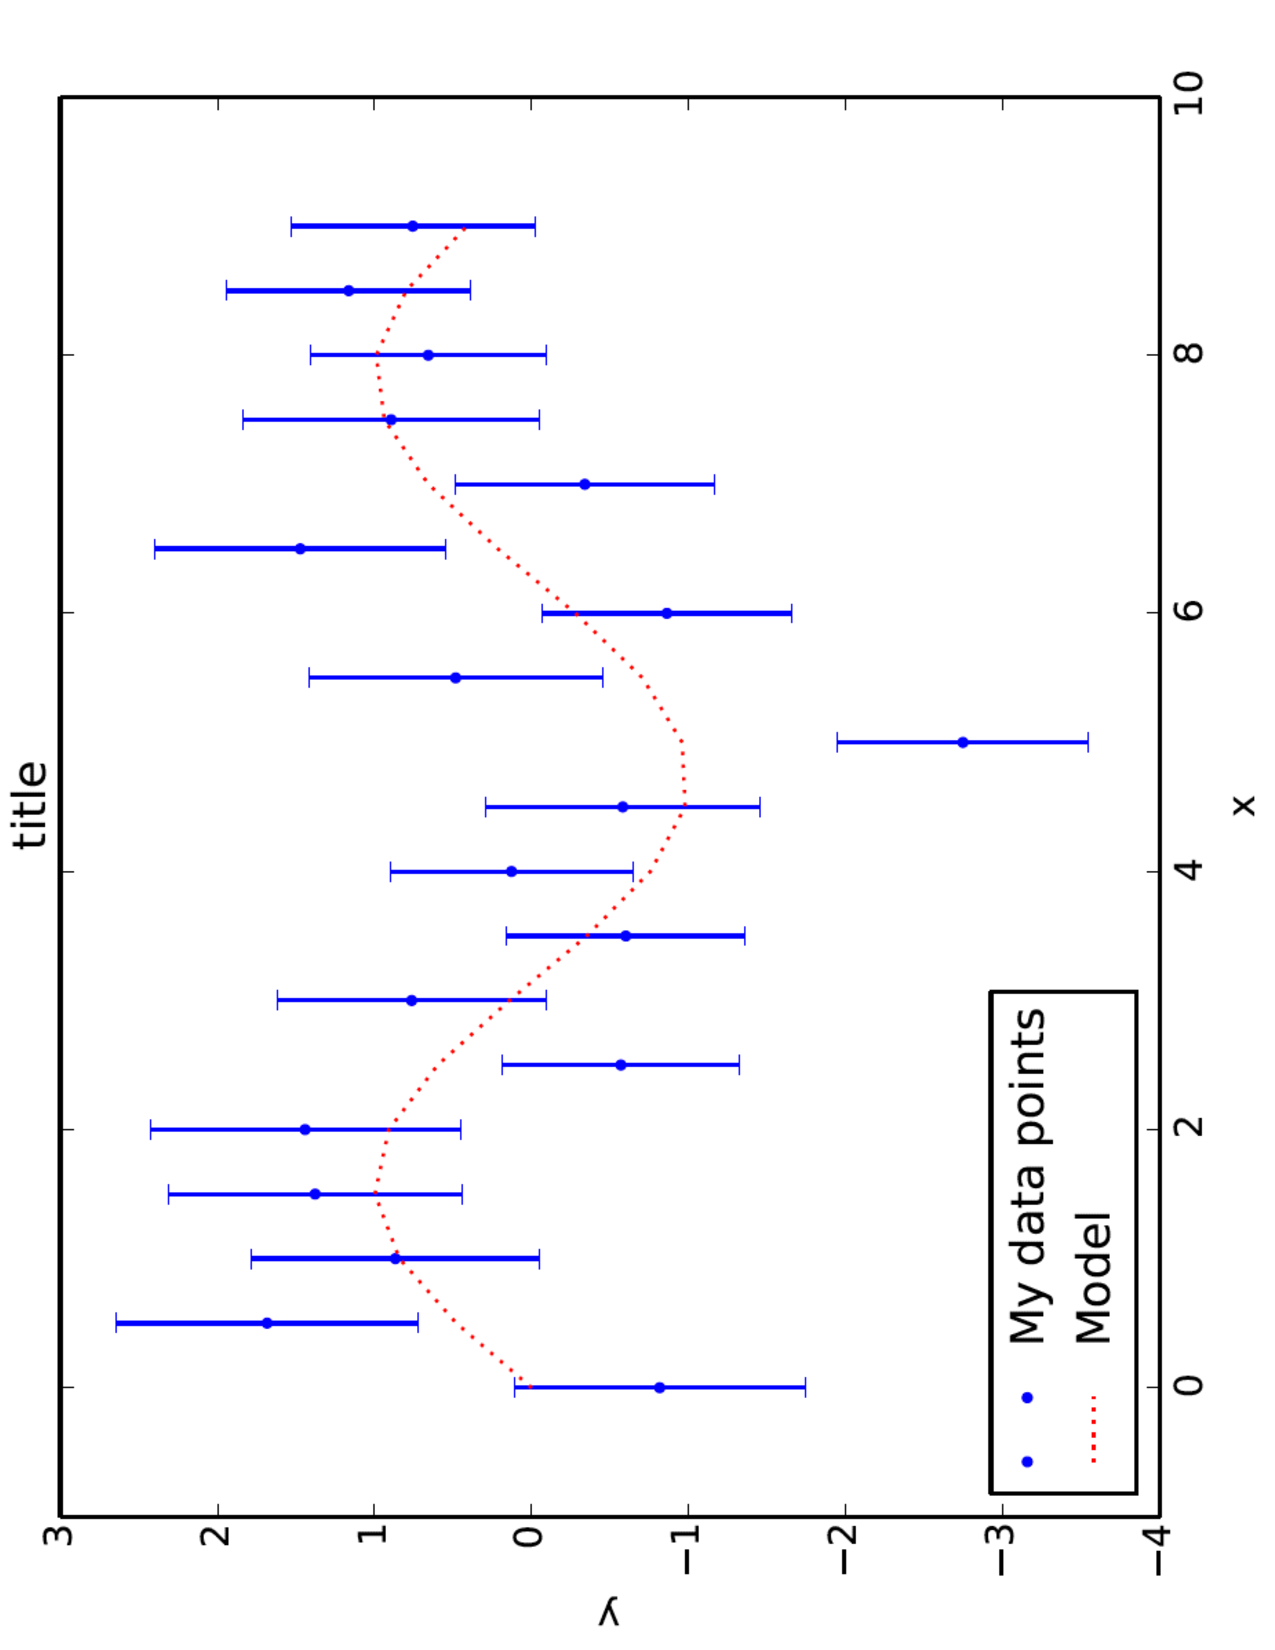
\includegraphics[angle=-90,width=8.5cm]{./figures/plot_sin}
\end{frame}

\begin{frame}[fragile,label=sec-3-10]{Using \verb~matplotlib.pyplot~}
% \snippetFile[Python]{src/example_matplotlib.py}

%\pause
%\includeSnippet{import}
%\pause
%\includeSnippet{make_sin}
%\pause
%\includeSnippet{plot_sin}
%
%\pause
%\includeSnippet{save_sin}
%\pause
%\includeSnippet{clear}
\end{frame}

\begin{frame}[fragile,label=sec-3-11]{Format characters}
 The format string is of the form \texttt{CM} (\texttt{C}olour\texttt{M}arker)
\def\hatSym{\texttt{$\hat{}$}}
\begin{center}
\begin{tabular}{|ll|ll|ll|}
\hline
\texttt{b} & \color{blue}blue & \texttt{-} & solid line & \texttt{.} & point\\
\texttt{g} & \color{green}green & \texttt{-}\texttt{-} & dashed line & \texttt{,} & pixel\\
\texttt{r} & \color{red}red & \texttt{:} & dotted line & \texttt{o} & circle\\
\texttt{c} & \color{cyan}cyan & \texttt{-.} & dot-dash line & \texttt{v} & triangle (down)\\
\texttt{m} & \color{magenta}magenta &  &  & \hatSym & triangle (up)\\
\texttt{y} & \color{yellow}yellow &  &  & \texttt{<} & triangle (left)\\
\texttt{k} & \color{black}black &  &  & \texttt{>} & triangle (right)\\
\texttt{w} & white &  &  &  & \\
\hline
\end{tabular}
\end{center}

There are more colours, but it's better to use the \texttt{color} keyword.  For markers, it's really better 
to use the \texttt{marker} and \texttt{linestyle} (abbreviation: \texttt{ls}) keywords
\end{frame}
\begin{frame}[fragile,label=sec-3-12]{Semi-\textit{OO} plotting with \verb~matplotlib~}
% \snippetFile[Python]{src/example_matplotlib.py}
%
%We can do the same thing using a \verb~figure~:
%\includeSnippet{makeFigure}
%\includeSnippet{plot_axes_sin}
\end{frame}

\begin{frame}[fragile,label=sec-3-13]{Jupyter (a.k.a. iPython) notebooks}
 We can run these commands in the browser with a command like:
\lstset{language=text,label= ,caption= ,numbers=none}
\begin{lstlisting}
$ jupyter notebook --no-browser src/notebooks/sin.ipynb
\end{lstlisting}
This provides a nice way of documenting your work.

See \url{http://jupyter.readthedocs.io/en/latest/install.html}
\end{frame}

\begin{frame}[fragile,label=sec-3-14]{Multi-panel plots}
 Once again, I need a \verb~figure~, and then 
the command to select the third sub-window out of a \verb~2x2~ set is
\lstset{language=Python,label= ,caption= ,numbers=none}
\begin{lstlisting}
figure.add_subplot(2, 2, 3)
\end{lstlisting}
\pause so I could say
\lstset{language=Python,label= ,caption= ,numbers=none}
\begin{lstlisting}
axes = figure.add_subplot(2, 2, 1)
# make a plot
axes = figure.add_subplot(2, 2, 2)
# make another plot
axes = figure.add_subplot(2, 2, 3)
# keep plotting
axes = figure.add_subplot(2, 2, 4)
# plot plot plot
\end{lstlisting}
But I'm lazy and I don't like duplicating \verb~2, 2~

\pause
Instead, I'll use a generator:
%\snippetFile[Python]{src/example_matplotlib.py}
%
%\pause
%\includeSnippet{subplots}
\end{frame}
\begin{frame}[label=sec-3-15]{Panel I: Histogram}
%\snippetFile[Python]{src/example_matplotlib.py}
%\pause
%\includeSnippet{makeFigure}
%\includeSnippet{subplots}
%\pause
%\includeSnippet{histogram}
\end{frame}

\begin{frame}[label=sec-3-16]{\quad}
\begin{center}
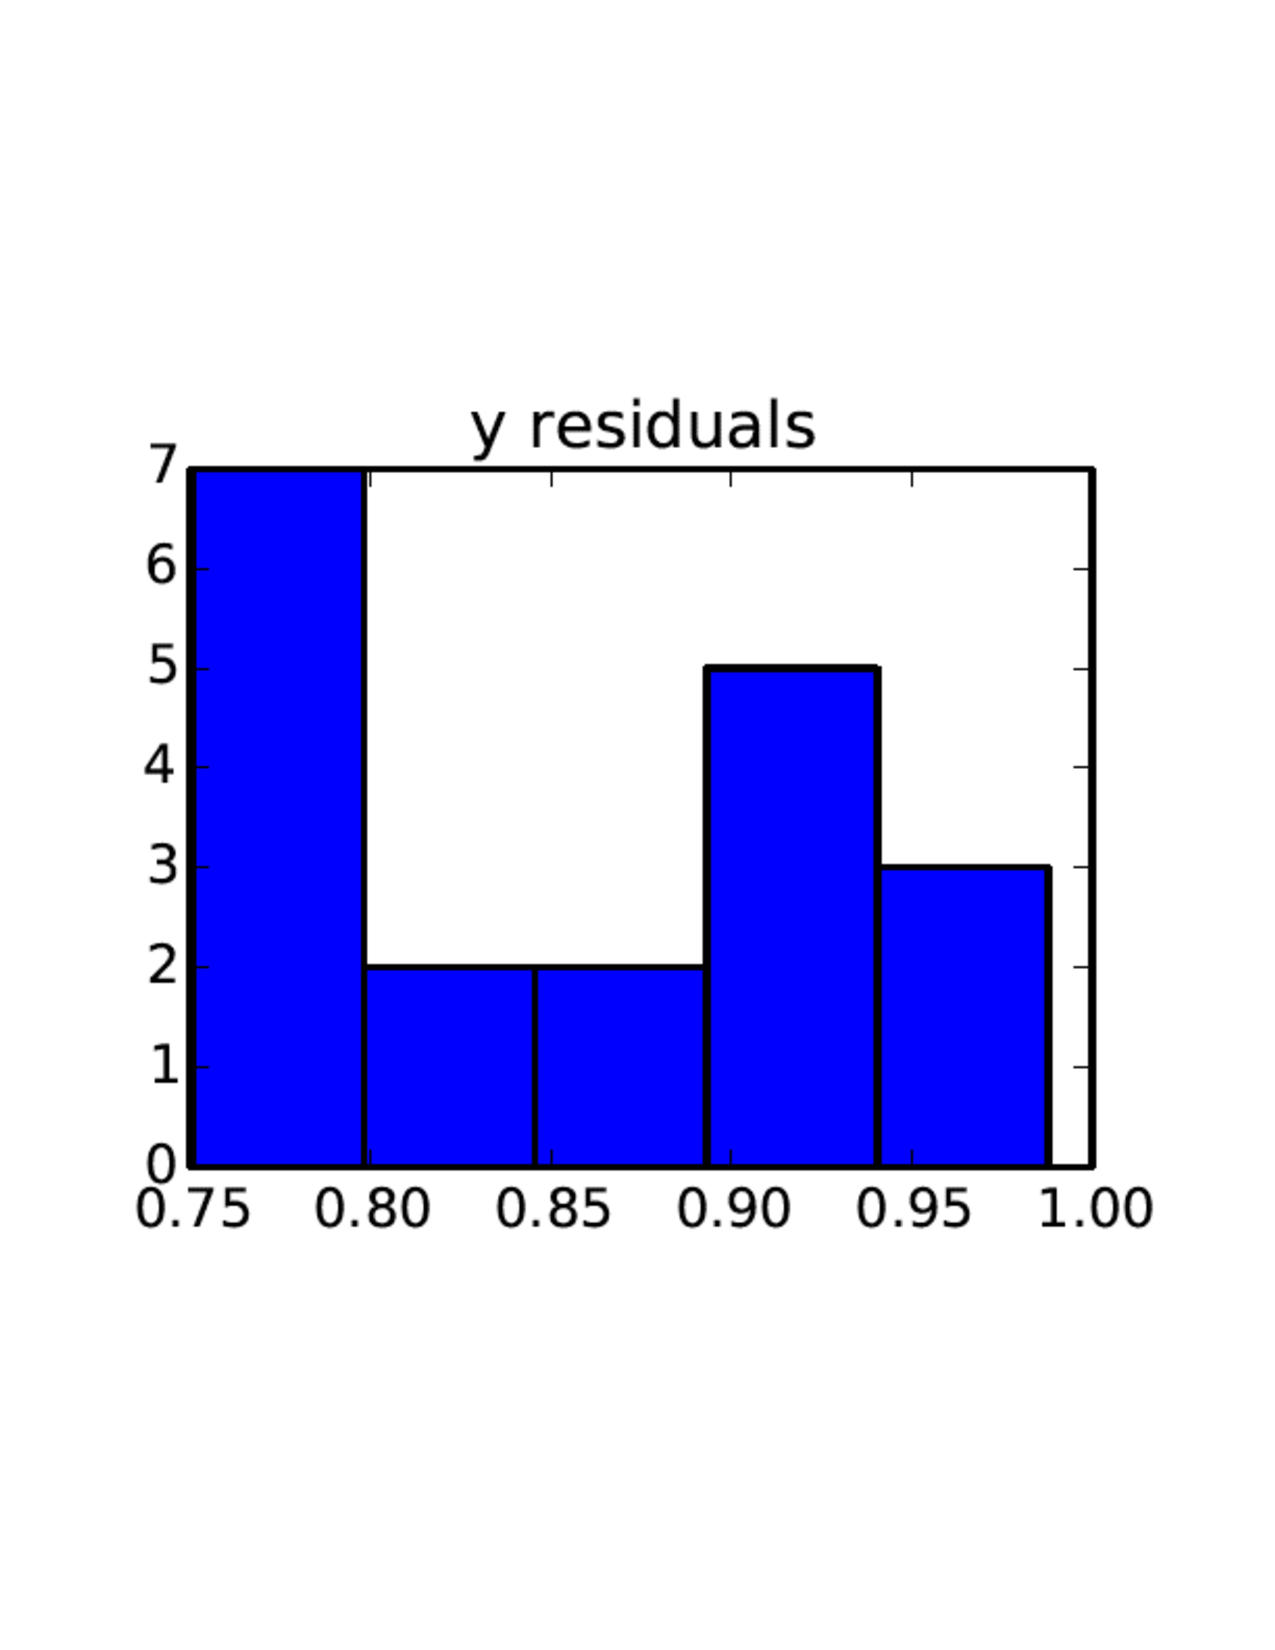
\includegraphics[width=5.5cm]{./figures/plot_histogram.pdf}
\end{center}
\pause
\vspace*{-1cm}
Hmm.  Not a good choice for the axis limits.
\end{frame}
\begin{frame}[label=sec-3-17]{Panel I: Histogram}
Let's fix those limits:
\includeSnippet{makeFigure}
\includeSnippet{subplots}
\includeSnippet{histogramII}
\end{frame}

\begin{frame}[label=sec-3-18]{\quad}
\begin{center}
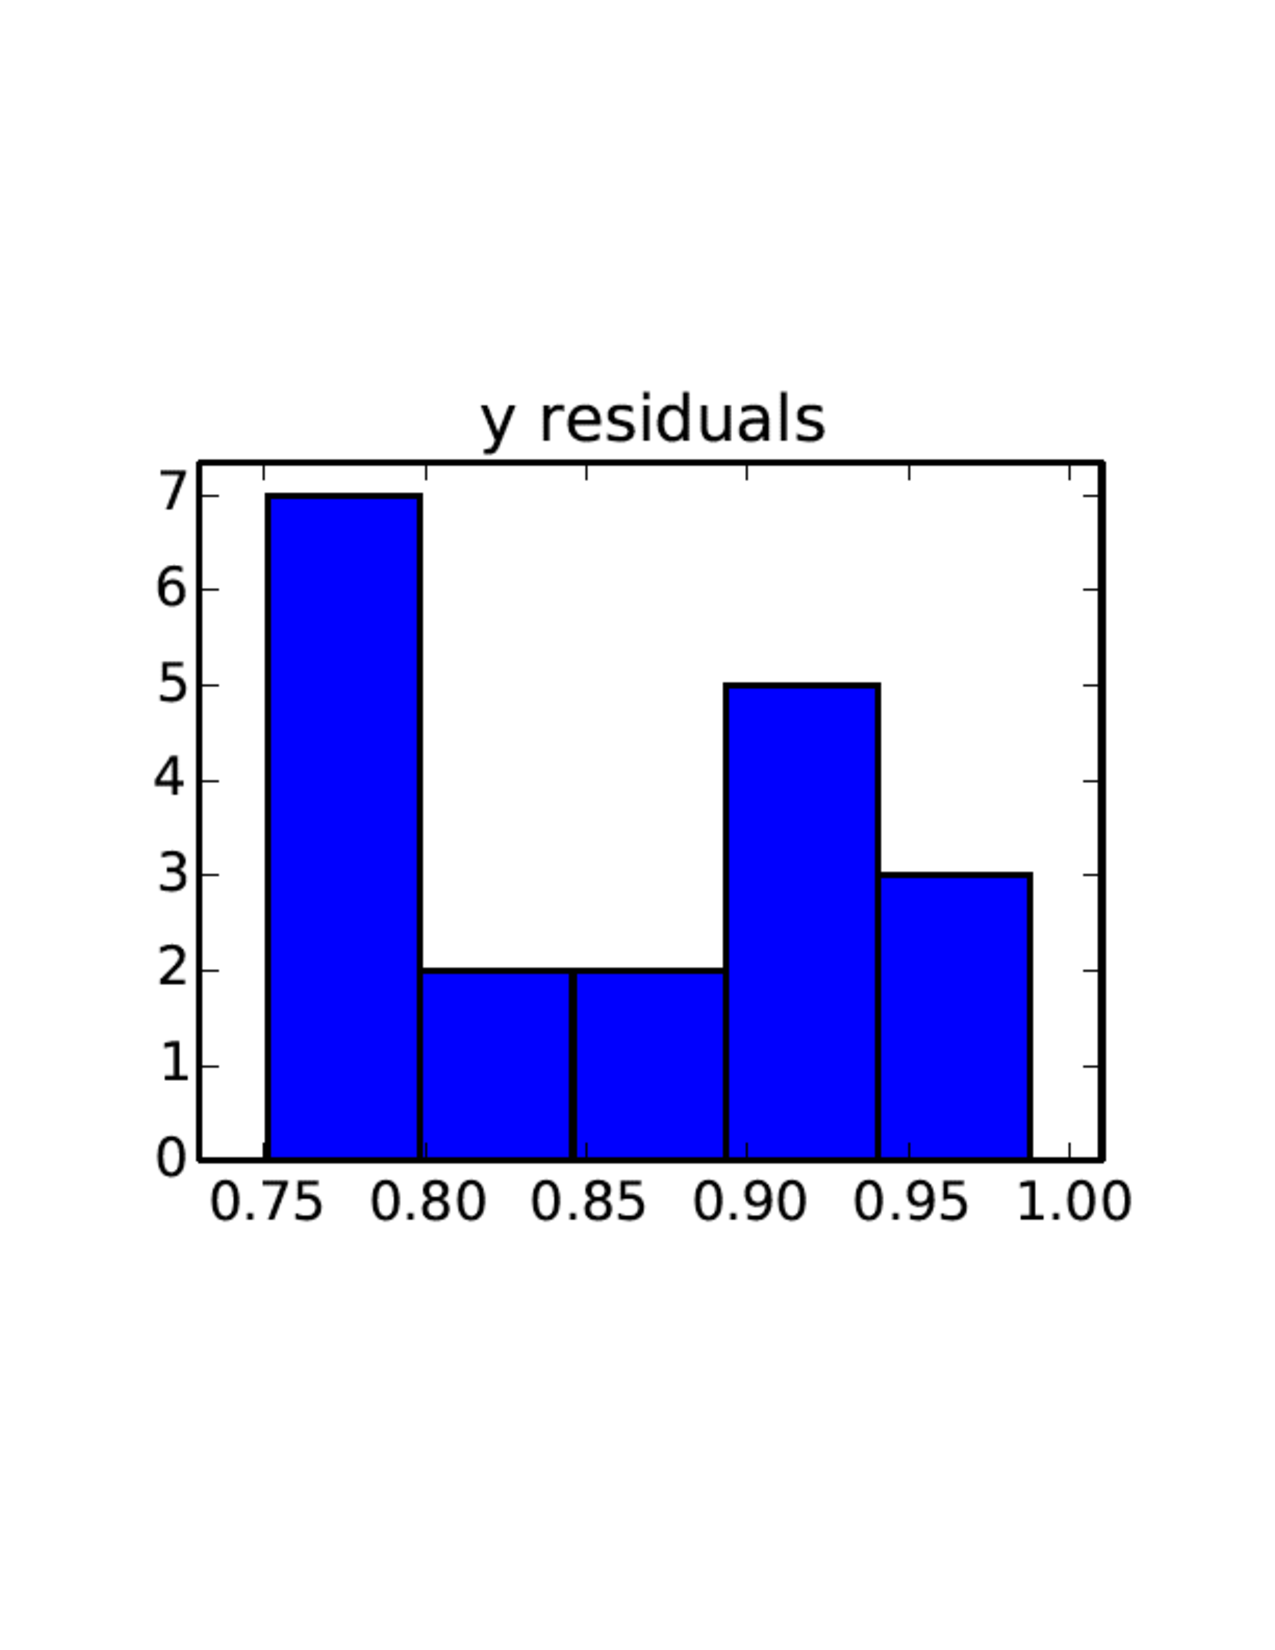
\includegraphics[width=5.5cm]{./figures/plot_histogramII.pdf}
\end{center}
\end{frame}
\begin{frame}[label=sec-3-19]{Panel II: Log-linear}
%\snippetFile[Python]{src/example_matplotlib.py}
%\pause
%\includeSnippet{log}
%\pause
%\includeSnippet{rhs_axis}
%\pause
%\includeSnippet{position_label}
\end{frame}
\begin{frame}[label=sec-3-20]{\quad}
\begin{center}
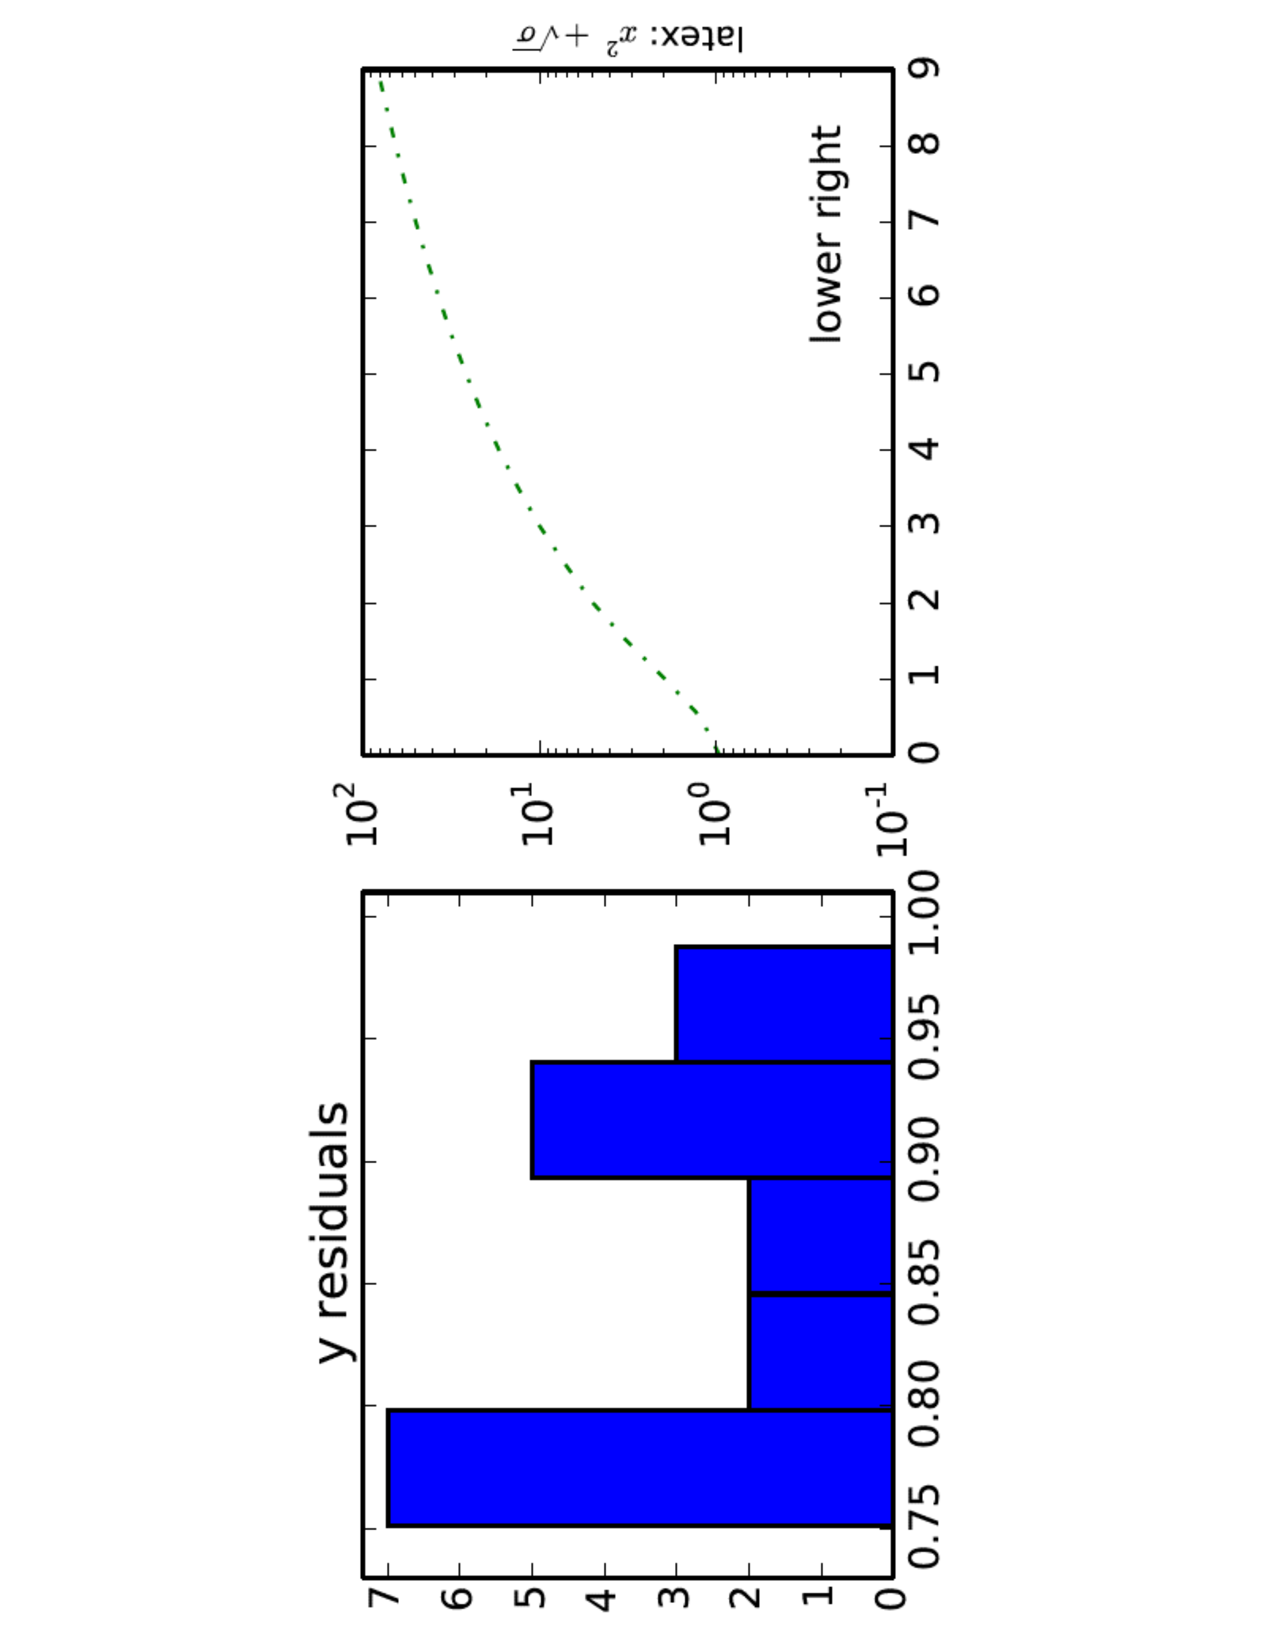
\includegraphics[angle=-90,width=10.5cm]{./figures/plot_log.pdf}
\end{center}
\end{frame}
\begin{frame}[label=sec-3-21]{Panel III: Scatter Plot}
%\snippetFile[Python]{src/example_matplotlib.py}
%\pause
%\includeSnippet{init_scatter}
%\pause
%\includeSnippet{plot_scatter}
\end{frame}

\begin{frame}[label=sec-3-22]{\quad}
\begin{center}
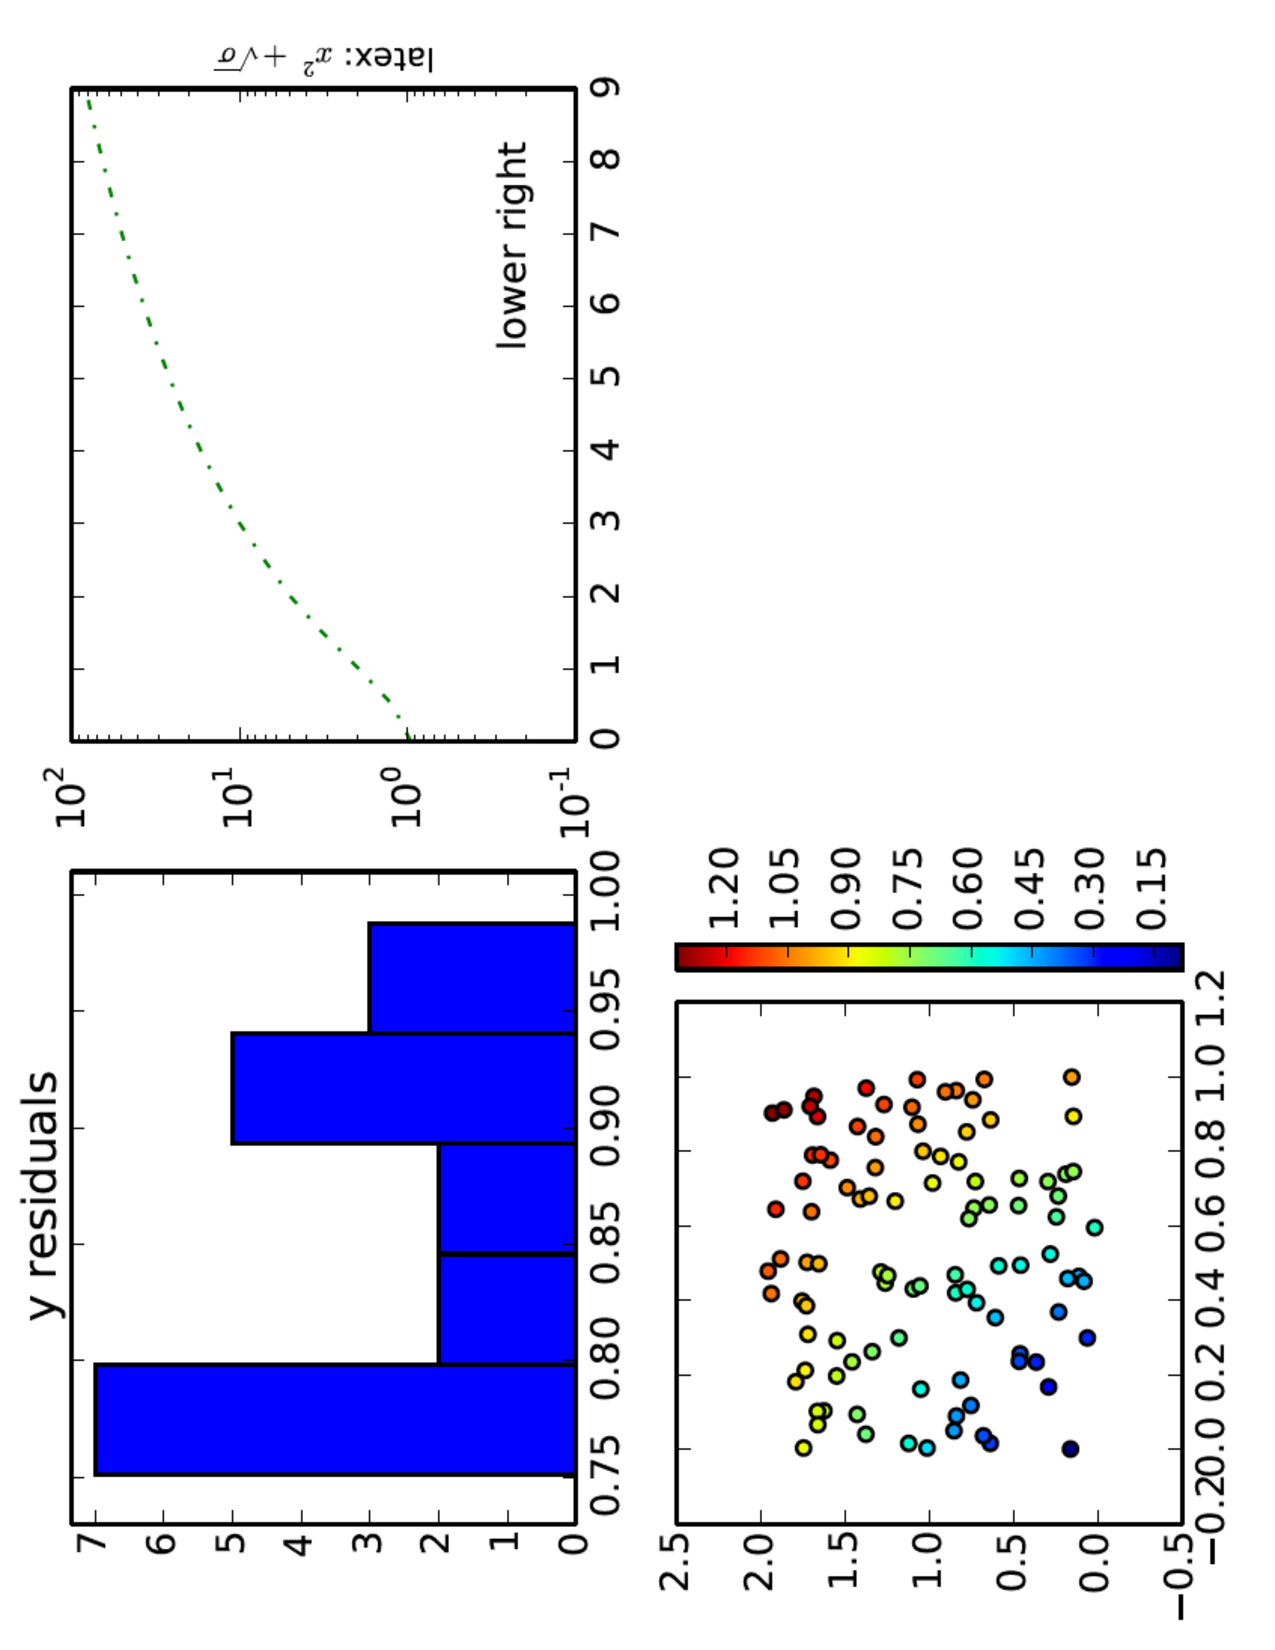
\includegraphics[angle=-90,width=8.5cm]{./figures/plot_scatter.pdf}
\end{center}
\end{frame}
\begin{frame}[label=sec-3-23]{Panel IV: Contours}
%\snippetFile[Python]{src/example_matplotlib.py}
%\pause
%\includeSnippet{init_contour}
%\pause
%\includeSnippet{plot_contour}
%\pause
%\includeSnippet{label_contour}
%\pause
%\includeSnippet{aspect}
%\pause
%\includeSnippet{ticklabel}

%\pause
%\includeSnippet{save_multi}
\end{frame}

\begin{frame}[label=sec-3-24]{\alert{plot\_multi.pdf}}
\begin{center}
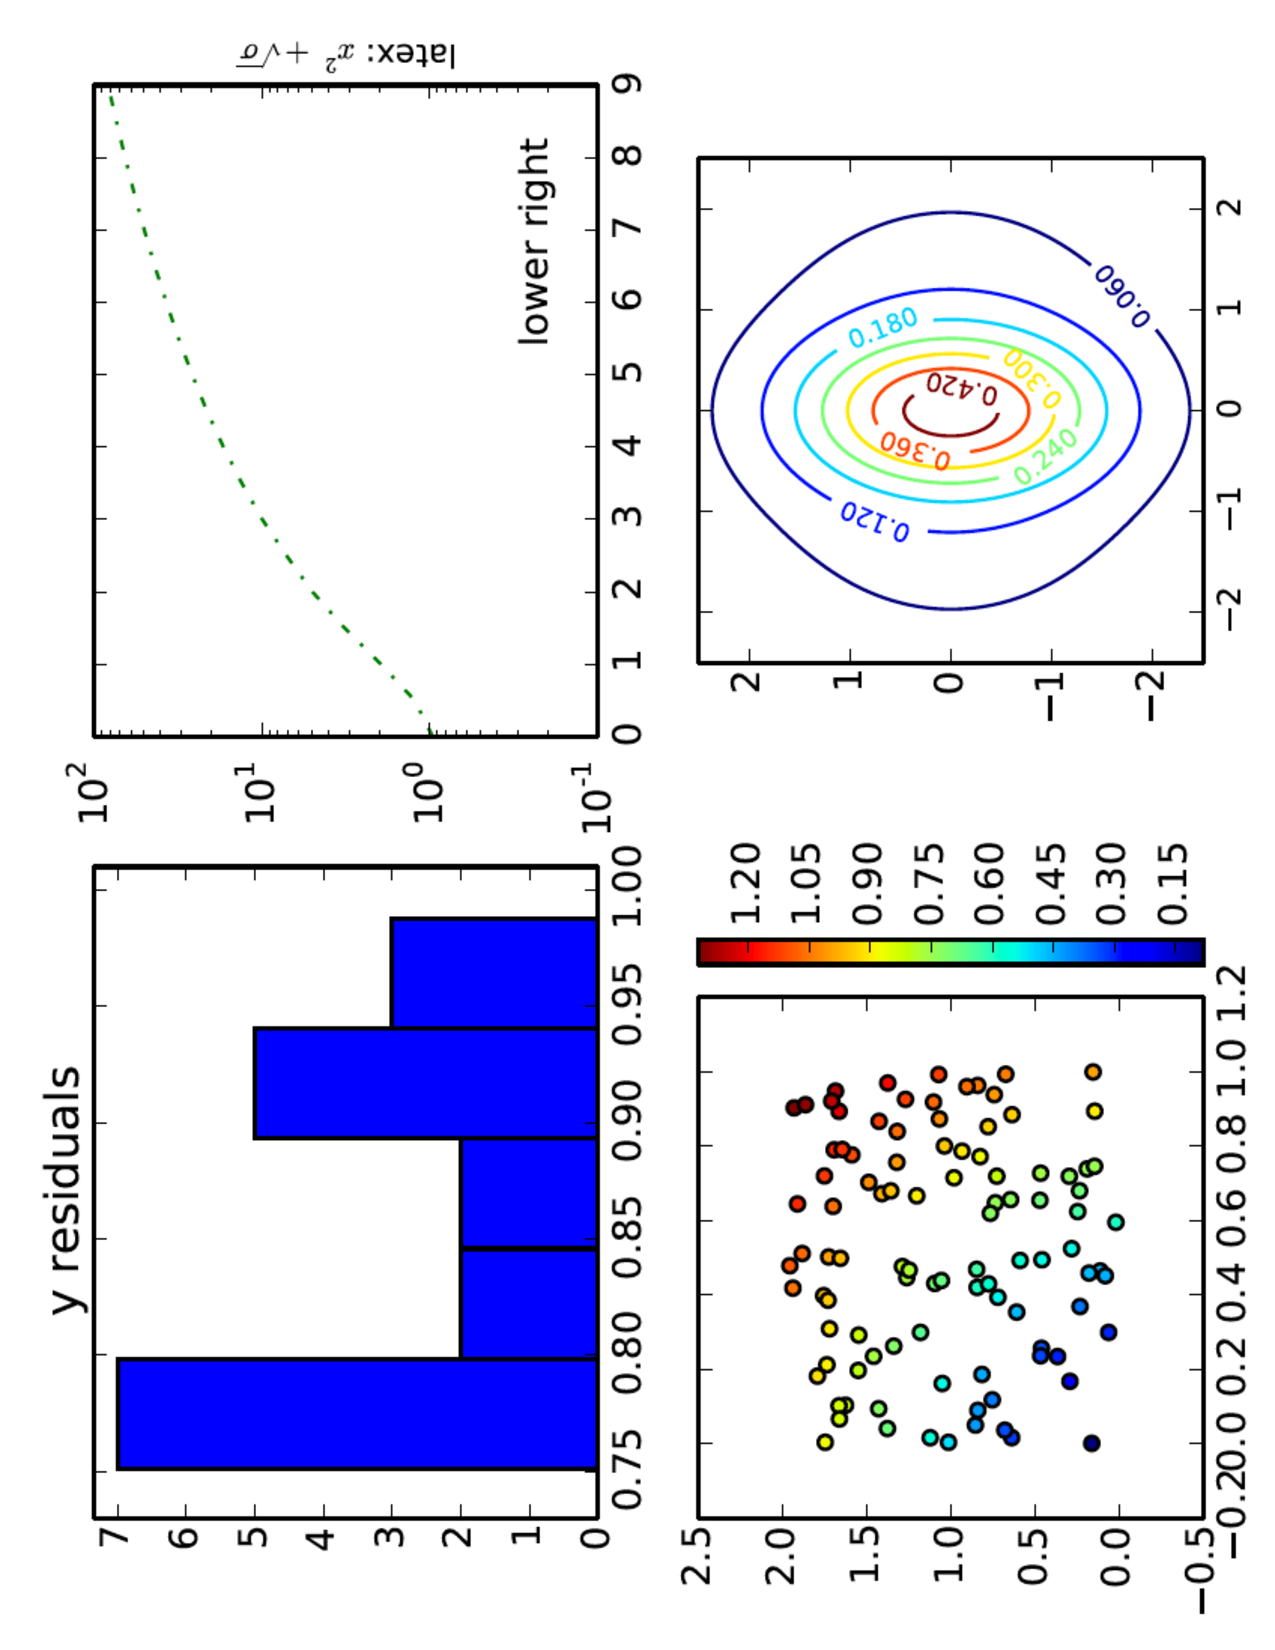
\includegraphics[angle=-90,width=8.5cm]{./figures/plot_multi.pdf}
\end{center}
\end{frame}
\begin{frame}[fragile,label=sec-3-25]{Non-interactive plotting}
 What if you just want to make a plot, and not worry about \verb~interactive~ and \verb~Qt~?  One
way is to use a \verb~canvas~:

%\snippetFile[Python]{src/example_matplotlib_nointer.py}
%
%\pause
%We needn't \verb~import pyplot~:
%and the command to make the \verb~figure~ is a little different:
%\includeSnippet{makeFigure}
%\pause
%The rest of the plotting is identical:
%\includeSnippet{plot_axes_sin}
%
%\pause
%And finally we use that \verb~canvas~:
%\includeSnippet{plotToCanvas}
\end{frame}

\begin{frame}[fragile,label=sec-3-26]{Array operations, \verb~numpy~}
 While the array library, \verb~numpy~, is not part of the python standard library it is widely available.
\begin{block}{NumPy home (but it's easier to get it from \emph{anaconda})}
\url{http://numpy.scipy.org}

\pause
\end{block}
\begin{block}{We used a few pieces of \verb~numpy~ in the \verb~matplotlib~ examples:}
\lstset{language=Python,label= ,caption= ,numbers=none}
\begin{lstlisting}
import numpy as np
\end{lstlisting}
\pause
\lstset{language=Python,label= ,caption= ,numbers=none}
\begin{lstlisting}
x = np.linspace(0.0, 9.0, 19)
model = np.sin(x)
\end{lstlisting}
\pause
\lstset{language=Python,label= ,caption= ,numbers=none}
\begin{lstlisting}
yerr = np.abs(y - model)
zs = np.sqrt(xs**2 + ys**2/4.0)
\end{lstlisting}
\pause
\lstset{language=Python,label= ,caption= ,numbers=none}
\begin{lstlisting}
np.random.seed(666)
xs = np.random.random(100)
y = np.random.normal(loc=model, scale=0.2)
\end{lstlisting}
\pause
\lstset{language=Python,label= ,caption= ,numbers=none}
\begin{lstlisting}
axis = np.linspace(-2.0, 2.0, 100)
X, Y = np.meshgrid(axis, axis)
\end{lstlisting}

\pause
The \verb~import numpy as np~ is common enough that it's what the \texttt{numpy} documentation assumes.
\end{block}
\end{frame}

\begin{frame}[fragile,label=sec-3-27]{\verb~numpy~ Arrays}
 \pause
\lstset{language=Python,label= ,caption= ,numbers=none}
\begin{lstlisting}
>>> x = np.linspace(0.0, 5.0, 11); print x
[ 0.   0.5  1.   1.5  2.   2.5  3.   3.5  4.   4.5  5. ]
\end{lstlisting}
\pause
We could have used \verb~arange~ (analogous to python's \verb~range~):
\lstset{language=Python,label= ,caption= ,numbers=none}
\begin{lstlisting}
>>> print np.arange(0.0, 5.1, 0.5)
[ 0.   0.5  1.   1.5  2.   2.5  3.   3.5  4.   4.5  5. ]
\end{lstlisting}
\pause
There's also
\lstset{language=Python,label= ,caption= ,numbers=none}
\begin{lstlisting}
>>> print np.zeros(4), np.ones(4), np.empty(4, dtype='i')
[0.  0.  0.  0.] [1.  1.  1.  1.] [9 0 18402543 1]
\end{lstlisting}
\pause
\lstset{language=Python,label= ,caption= ,numbers=none}
\begin{lstlisting}
>>> x = np.arange(5); print np.multiply.outer(x, x)
[[ 0  0  0  0  0]
 [ 0  1  2  3  4]
 [ 0  2  4  6  8]
 [ 0  3  6  9 12]
 [ 0  4  8 12 16]]
\end{lstlisting}
\end{frame}
\begin{frame}[fragile,label=sec-3-28]{\verb~numpy~ Mathematical functions}
 \pause
\lstset{language=Python,label= ,caption= ,numbers=none}
\begin{lstlisting}
>>> x = np.arange(5)
>>> y = np.sin(x); print y
[ 0.          0.84147098  0.90929743  0.14112001 -0.7568025 ]
\end{lstlisting}
There are lots of other mathematical builtins (\verb~sin~, \verb~cos~, \verb~tan~, \verb~arcsin~, \verb~arctan2~, \verb~abs~, \verb~sqrt~, \ldots{})
\pause
\lstset{language=Python,label= ,caption= ,numbers=none}
\begin{lstlisting}
>>> print zip(x, y)
[(0, 0.0), (1, 0.8414709848078965), (2, 0.90929742682568171),
 (3, 0.14112000805986721), (4, -0.7568024953079282)]
\end{lstlisting}
\pause
\lstset{language=Python,label= ,caption= ,numbers=none}
\begin{lstlisting}
>>> print "\n".join(("%d %6.3f" % z for z in zip(x, y)))
0  0.000
1  0.841
2  0.909
3  0.141
4 -0.757
\end{lstlisting}
(OK, so that's a python, not \verb~numpy~, trick)
\end{frame}

\begin{frame}[fragile,label=sec-3-29]{\verb~numpy~ Random Numbers}
 \pause
\lstset{language=Python,label= ,caption= ,numbers=none}
\begin{lstlisting}
>>> np.random.seed(666)
>>> np.random.random(10)
array([ 0.70043712,  0.84418664,  0.67651434,  0.72785806,  0.95145796,
        0.0127032 ,  0.4135877 ,  0.04881279,  0.09992856,  0.50806631])
\end{lstlisting}
(\emph{n.b.} I didn't say \verb~print~, so I got the \verb~repr~ not the \verb~str~ value of the result)
\pause
\lstset{language=Python,label= ,caption= ,numbers=none}
\begin{lstlisting}
>>> print np.random.normal(loc=np.arange(5), scale=0.2)
[-0.2177586   0.88484585  1.66341985  3.04583705  3.64867496]
>>> print np.random.normal(np.arange(5), 0.2)
[ 0.16892652  1.05544397  2.17058031  3.03891992  4.26212754]
\end{lstlisting}
The two calls are identical, but the random numbers are (of course) different.
\end{frame}
\begin{frame}[fragile,label=sec-3-30]{\verb~numpy~ in n-D}
 \pause
\lstset{language=Python,label= ,caption= ,numbers=none}
\begin{lstlisting}
>>> axis = np.linspace(-2.0, 2.0, 5)
>>> X, Y = np.meshgrid(axis, axis)
>>> print X
[[-2. -1.  0.  1.  2.]
 [-2. -1.  0.  1.  2.]
 [-2. -1.  0.  1.  2.]
 [-2. -1.  0.  1.  2.]
 [-2. -1.  0.  1.  2.]]
>>> print Y
[[-2. -2. -2. -2. -2.]
 [-1. -1. -1. -1. -1.]
 [ 0.  0.  0.  0.  0.]
 [ 1.  1.  1.  1.  1.]
 [ 2.  2.  2.  2.  2.]]
\end{lstlisting}
\pause
\lstset{language=Python,label= ,caption= ,numbers=none}
\begin{lstlisting}
>>> print np.cos(X)*np.sin(Y)
[[ 0.37840125 -0.4912955  -0.90929743 -0.4912955   0.37840125]
 [ 0.35017549 -0.45464871 -0.84147098 -0.45464871  0.35017549]
 [-0.          0.          0.          0.         -0.        ]
 [-0.35017549  0.45464871  0.84147098  0.45464871 -0.35017549]
 [-0.37840125  0.4912955   0.90929743  0.4912955  -0.37840125]]
\end{lstlisting}
\pause
\lstset{language=Python,label= ,caption= ,numbers=none}
\begin{lstlisting}
>>> print np.fft.fft(X)*np.sin(Y)
[[-0.00000000+0.j          2.27324357-3.12885135j  2.27324357-0.73862161j
   2.27324357+0.73862161j  2.27324357+3.12885135j]
 [-0.00000000+0.j          2.10367746-2.89546363j  2.10367746-0.68352624j
   2.10367746+0.68352624j  2.10367746+2.89546363j]
 [ 0.00000000+0.j         -0.00000000+0.j         -0.00000000+0.j
   0.00000000-0.j          0.00000000-0.j        ]
...
\end{lstlisting}
\end{frame}

\begin{frame}[fragile,label=sec-3-31]{\verb~numpy~ indexing with Boolean arrays}
 You aren't restricted to using scalars as array indexes:
\lstset{language=Python,label= ,caption= ,numbers=none}
\begin{lstlisting}
>>> x = np.arange(-4, 5); print x
[-4 -3 -2 -1  0  1  2  3  4]
>>> i = x**2 > 4
>>> print i
[ True  True False False False False False  True  True]
>>> print x[i]
[-4 -3  3  4]
\end{lstlisting}
\pause
\lstset{language=Python,label= ,caption= ,numbers=none}
\begin{lstlisting}
>>> x[i] = 10 + np.abs(x[i])
>>> print x
[14 13 -2 -1  0  1  2 13 14]
\end{lstlisting}
\pause
\lstset{language=Python,label= ,caption= ,numbers=none}
\begin{lstlisting}
>>> I = np.array([2, 7])
>>> print x[I]
[-2 13]
\end{lstlisting}
\end{frame}

%\begin{frame}[fragile,label=sec-3-32]{Plotting and Extended Indexing}
% Here's another example

%\snippetFile[Python]{src/example_matplotlib.py}

%\includeSnippet{plot_where}
%The \verb~np.where~ is like C/\CPP's \verb~?:~ operator.
%\pause
%\vspace*{-2mm}
%\begin{center}
%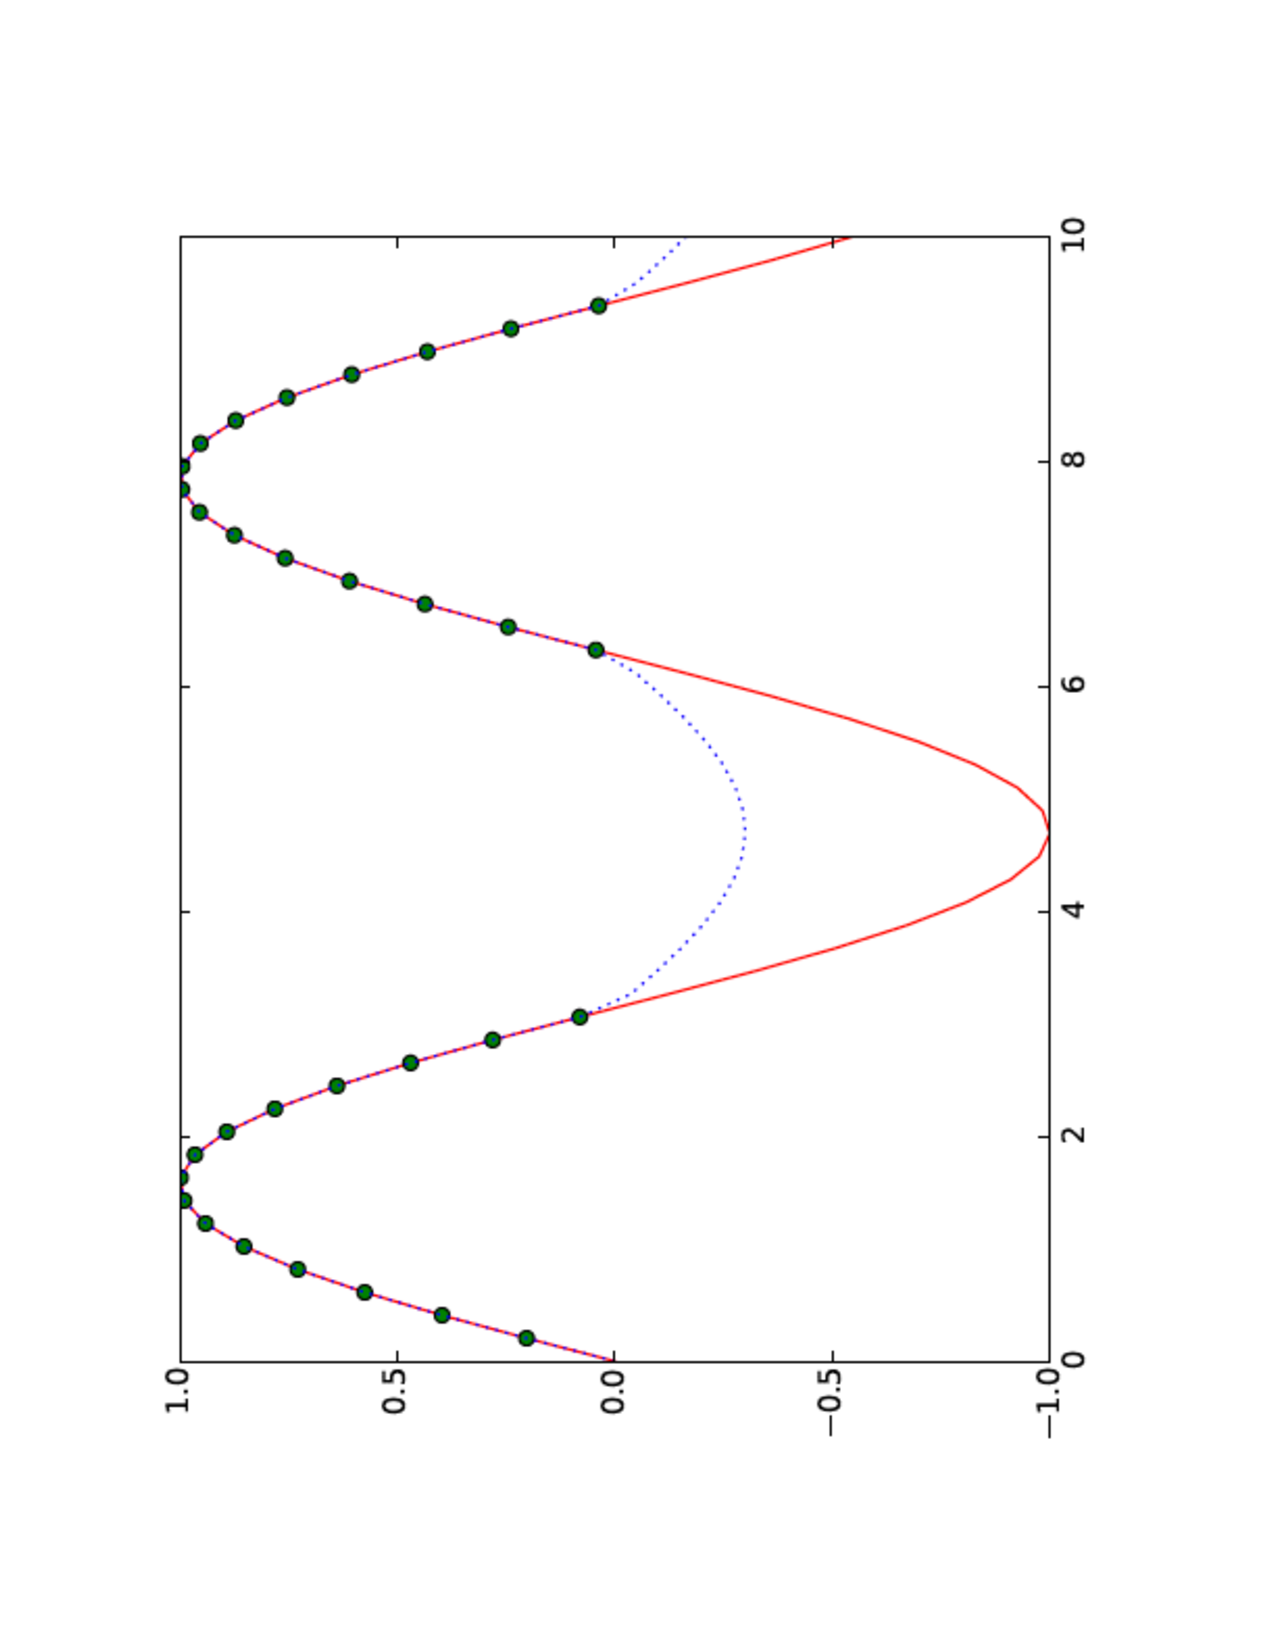
\includegraphics[width=5.5cm]{figures/plot_where}
%\end{center}
%\end{frame}

\begin{frame}[fragile,label=sec-3-33]{\verb~numpy~ Linear Algebra}
 \pause
\lstset{language=Python,label= ,caption= ,numbers=none}
\begin{lstlisting}
>>> n = 3; i = np.arange(n); M = np.zeros((n,n))
>>> M[(i,i)] = i + 1; print M
[[ 1.  0.  0.]
 [ 0.  2.  0.]
 [ 0.  0.  3.]]
>>> np.linalg.inv(M)
array([[ 1.        ,  0.        ,  0.        ],
       [ 0.        ,  0.5       ,  0.        ],
       [ 0.        ,  0.        ,  0.33333333]])
\end{lstlisting}

\pause
\lstset{language=Python,label= ,caption= ,numbers=none}
\begin{lstlisting}
>>> M = np.matrix(M)
>>> U, s, Vt = np.linalg.svd(M)
>>> U * np.diag(s) * Vt                   # should == M
matrix([[ 1.,  0.,  0.],
        [ 0.,  2.,  0.],
        [ 0.,  0.,  3.]])
\end{lstlisting}

\pause
Traps await the unwary:
\lstset{language=Python,label= ,caption= ,numbers=none}
\begin{lstlisting}
>>> M = np.zeros((n,n)); M[(i,i)] = i + 1
>>> U, s, Vt = np.linalg.svd(M)
>>> U * np.diag(s) * Vt
array([[ 0.,  0.,  0.],
       [ 0.,  2.,  0.],
       [ 0.,  0.,  0.]])
\end{lstlisting}
Uh oh; that's an element-by-element product.
\pause
An \verb~array~ is not a \verb~matrix~; you have to say
\lstset{language=Python,label= ,caption= ,numbers=none}
\begin{lstlisting}
>>> U.dot(np.diag(s)).dot(Vt)
\end{lstlisting}
\end{frame}


\begin{frame}[fragile,label=sec-3-34]{\verb~numpy~ Linear Algebra}
 Beware: vectors are treated differently from matrices.  The vector \verb~x~ is the
same as the vector \verb~x.T~:
\lstset{language=Python,label= ,caption= ,numbers=none}
\begin{lstlisting}
>>> x = np.array((1, 2))
>>> x
array([1, 2])
>>> x.T
array([1, 2])
>>> np.dot(x, x.T)
5
>>> np.dot(x.T, x)
5
\end{lstlisting}
\pause
If you want to distinguish between row vectors and column vectors, need to use a
$1\times n$ or $n\times 1$ matrix:
\lstset{language=Python,label= ,caption= ,numbers=none}
\begin{lstlisting}
>>> x.resize(1,2)
>>> x
array([[1, 2]])
>>> x.T
array([[1],
       [2]])
>>> np.dot(x, x.T)
array([[5]])
>>> np.dot(x.T, x)
array([[1, 2],
       [2, 4]])
\end{lstlisting}
\end{frame}

\begin{frame}[fragile,label=sec-3-35]{\verb~numpy~ Linear Algebra}
 If you use a \verb~matrix~, you don't need to use \verb~dot~:
\lstset{language=Python,label= ,caption= ,numbers=none}
\begin{lstlisting}
>>> v = np.matrix((1, 2))
>>> v * v.T
matrix([[5]])
>>> v.T * v
matrix([[1, 2],
        [2, 4]])
\end{lstlisting}

\pause
A future version of python will support \verb~U @ np.diag(s) @ Vt~
with \verb~@~ meaning, "matrix multiply".
\pause
This does not remove the confusion between vectors and matrices, however: it is
merely a shorthand for \verb~U.dot(np.diag(s)).dot(Vt)~.
\end{frame}

%FIXME
%add ufuncs, and dont say indexing, say boolean indexing
\begin{frame}[fragile,label=sec-3-36]{Other \verb~numpy~ capabilities}
 \verb~numpy~ has lots of libraries:
\begin{itemize}
\item FFTs
\item Linear algebra
\item Statistics
\item \emph{etc.}
\end{itemize}

\pause
I used the statistics package in analyzing the course questionnaire:
\lstset{language=Python,label= ,caption= ,numbers=none}
\begin{lstlisting}
  cov = np.corrcoef(data, rowvar=False)
  for i in range(len(cov[0])):
     print "%6.3f" np.mean(data[:, i]), \
           " ".join(["%6.3f" % x for x in cov[i]])
\end{lstlisting}

\pause
The \verb~scipy~ package adds many more:
\begin{itemize}
\item N-dimensional image convolution
\item Interpolation
\item Sparse linear algebra (\emph{e.g.} \verb~3M x 5k~ least-squares problems)
\item Optimization
\item \emph{etc.}
\end{itemize}
\end{frame}

\section{Beyond Libraries}
\label{sec-4}
\begin{frame}[label=sec-4-1]{Embedding C/\CPP/Fortran in python}
One extremely powerful technique is to wrap your own code in python, a topic that we'll cover 
later in the course.  To whet your appetite, here's some analysis code that I wrote four years ago last week:
\end{frame}
% Emacs 24.5.1 (Org mode 8.2.7c)
\end{document}
